%%%%%%%%%%%%%%%%%%%%%%%%%%
%%%                    %%%
%%%      Preamble      %%%
%%%                    %%%
%%%%%%%%%%%%%%%%%%%%%%%%%%

\documentclass[12pt]{article}

% Language setting
% Replace `english' with e.g. `spanish' to change the document language
\usepackage[english]{babel}

% Set page size and margins
% Replace `letterpaper' with`a4paper' for UK/EU standard size
\usepackage[letterpaper,top=2cm,bottom=3cm,left=3cm,right=2.5cm,marginparwidth=1.75cm]{geometry}
    \topskip        =   20pt
    \parskip        =   0pt
    \parindent      =   20 pt
    \baselineskip   =   15pt
    
% line spacing
\usepackage{setspace}
    \onehalfspacing

% Useful packages
\usepackage{amssymb, amsfonts, amsmath}
\usepackage{graphicx}
\usepackage[hidelinks, hypertexnames=false]{hyperref}
\usepackage{bm}
\usepackage{xcolor}
\usepackage{adjustbox}
\usepackage[labelfont=bf]{caption}            % to reset the headers of tables 
\usepackage{rotating}           % for sidewaystable
\usepackage{float}
\usepackage{array}
\usepackage{nameref}

%\numberwithin{table}{section}    % reset the Table numbering for each section

%% these three are essential for estout
\usepackage{booktabs}  % neatly formatting lines
\usepackage{threeparttable}    
\usepackage{dcolumn}    % aligning decimals
    \newcolumntype{d}[1]{D{.}{.}{#1}}

% New font package
%\usepackage{newpxtext}
\usepackage{mathptmx}

% *****************************************************************
% Estout LaTeX wrapper
% *****************************************************************

 \makeatletter %this is needed to allow latex to revert to prior installations to fix noalign error
\let\estinput=\@@input % define a new input command so that we can still flatten the document

\newcommand{\estwide}[3]{
		\vspace{.75ex}{
			%\textsymbols% Note the added command here
			\begin{tabular*}
			{\textwidth}{@{\hskip\tabcolsep\extracolsep\fill}l*{#2}{#3}}
			\toprule
			\estinput{#1}
			\bottomrule
			\addlinespace[.75ex]
			\end{tabular*}
			}
		}	

\newcommand{\estfit}[3]{
        \vspace{.75ex}{
            \resizebox{\textwidth}{!}{%
            \begin{tabular}{l*{#2}{#3}}
            \toprule
            \estinput{#1}
            \bottomrule
            \addlinespace[.75ex]
            \end{tabular}}
            }
        }

\newcommand{\estauto}[3]{
		\vspace{.75ex}{
			%\textsymbols% Note the added command here
			\begin{tabular}{l*{#2}{#3}}
			\toprule
			\estinput{#1}
			\bottomrule
			\addlinespace[.75ex]
			\end{tabular}
			}
		}

% Allow line breaks with \\ in special cells
\newcommand{\specialcell}[2][c]{%
    \begin{tabular}[#1]{@{}c@{}}#2\end{tabular}
}

\usepackage{comment}
\usepackage{lscape}
\usepackage[round]{natbib}

\usepackage{titling} % Required for custom title

%%%%%%%%%%% End of wrapper %%%%%%%%%%%%%%%%%%%%%

%%%%%%%%%%%%%%%%%%%%%%%%%%
%%%                    %%%
%%%      Document      %%%
%%%                    %%%
%%%%%%%%%%%%%%%%%%%%%%%%%%


\title{\large\textbf{Citizen Monitoring and Bureaucratic Output: \\ Evidence from the Bureau of Indian Affairs} 
\thanks{We thank John Bitzan, Justin Frye, Cesar Martinelli, Richard Monette, Nicola Maaser, and Jessica Shoemaker for their helpful comments and suggestions.}}

\author{
    Olga Shanks\\
    Southeastern Louisiana University\\
    olga.shanks@southeastern.edu\\
    \vspace{-2mm}\\
    Thomas Stratmann\\
    George Mason University\\
    tstratma@gmu.edu
}

\date{July 2026}

\begin{document}
\maketitle


\thispagestyle{empty}
{\singlespacing % Start single spacing
\begin{abstract}\noindent
We study how the distribution of beneficiary stakes affects the output a bureaucracy secures when monitoring is costly and shared. The model treats monitoring the agency as a public good among beneficiaries. When beneficiaries are more numerous or stakes are more equal, each captures less of the return from monitoring. Aggregate monitoring falls, bureaucratic effort falls, and output declines. We test this prediction using administrative data on agricultural leases for co-owned allotted trust land administered by the Bureau of Indian Affairs (BIA). Lease income per trust acre measures the output the BIA secures for owners, who receive income in proportion to inherited ownership interests. Because unobserved land productivity, original allottee characteristics, and family histories may affect both ownership fractionation and lease income, we instrument fractionation with the earliest and latest qualifying probate orders approved no later than the lease effective date. In the preferred instrumental-variables specification, reducing the largest owner's share from 40 percent to 20 percent lowers lease income per trust acre by about 14 percent, compared with 2 to 3 percent in least-squares estimates. Additional descriptive patterns are consistent with the monitoring interpretation. The evidence shows how dispersed claims can weaken oversight of a shared bureaucratic agent.



\vspace{\baselineskip}
\noindent
\textbf{Keywords:} Bureaucracy, Public Goods, Citizen Monitoring, Bureau of Indian Affairs\\
\textbf{JEL Codes:} H42, D73, D23

\end{abstract}
} % End single spacing

\defcitealias{GAO1999}{the U.S. Government Accountability Office}
\defcitealias{GAO2015}{GAO}
\defcitealias{GAO2019}{GAO}
\defcitealias{BIA2012}{BIA}
\defcitealias{BIA2006Ch1}{BIA}
\defcitealias{BIA2006Ch2}{BIA}
\defcitealias{BIA2023}{BIA}
\defcitealias{Title25}{Title 25 §162}


\pagebreak
\setcounter{page}{1}


\section{Introduction}

How does the distribution of beneficiaries' stakes affect a bureaucracy's output? Bureaucrats often have discretion over how much effort to devote to individual claims, services, and enforcement tasks. Political principals provide broad oversight, but the people most affected by an agency's decisions often monitor those decisions directly by attending hearings, contacting the agency, filing complaints, or writing to decision-makers \citep{Wilson1989}. Monitoring is costly. When one bureaucratic decision produces a shared output, each beneficiary captures only part of the gain from monitoring and has reason to leave that monitoring to others.

We formalize this logic as a public-goods problem in monitoring. Beneficiaries receive shares of a common bureaucratic output and may make costly monitoring contributions that raise bureaucratic effort. The model predicts that dispersed claims reduce monitoring and output: more beneficiaries or more equal stakes lower each beneficiary's private return to monitoring. With unequal stakes and common monitoring costs, the largest stake determines the equilibrium monitoring contribution, up to ties. Lower monitoring costs raise monitoring and output because a given stake supports more agency oversight.

We test these predictions using administrative records on agricultural leases for co-owned allotted trust land administered by the Bureau of Indian Affairs (BIA). Inheritance has divided many tracts into undivided ownership interests, meaning fractional claims to the whole tract rather than demarcated physical pieces. Owners receive lease income in proportion to these inherited interests, so they are the beneficiaries in the model. We call the dispersion of their ownership shares ownership fractionation. When an owner contacts the BIA, supplies information about land use, requests a higher rent, or monitors compliance, all owners benefit through the same tract-level lease income. Lease income per trust acre therefore measures the output the BIA secures for owners on the trust portion of the tract, while ownership shares determine owners' incentives to monitor the agency.

Ownership structure is endogenous. Unobserved land productivity, original allottee characteristics, and family histories may affect both the ownership structure a tract inherits and the lease income it commands. Our main design instruments ownership fractionation with the earliest and latest qualifying probate orders approved no later than the lease effective date. Probate orders divide a deceased owner's undivided interest among heirs, so their timing predicts ownership structure. Conditional on reservation and lease-signing year fixed effects, the design compares tracts in the same reservation rental market whose probate histories unfolded at different times. Identification requires that the remaining probate-timing variation affect lease income only through ownership fractionation. The probate-timing variables strongly predict fractionation, and we assess the main threats to exclusion using the lease-effective-date instrument construction, allotment-cohort controls within reservation, soil-productivity balance tests, weak-instrument-robust inference, and leave-one-reservation-out checks. The preferred IV sample excludes the Crow Reservation because its competency-leasing regime can place some agricultural leases outside the BIA bargaining channel central to the model. Estimates that include that reservation are transparency comparisons.

The main instrumental-variables estimate shows that ownership fractionation lowers lease income per trust acre. In the preferred specification, reducing the largest owner's share from 40 percent to 20 percent lowers income by about 14 percent. The corresponding least-squares estimates imply a decline of about 2 to 3 percent. The larger IV estimate is consistent with omitted-variable bias pushing least squares toward zero: if lower-productivity land both commands lower rents and leaves poorer families with fewer surviving heirs, then less fractionated tracts look low-income for reasons unrelated to monitoring. Because the IV estimate is local to tracts whose ownership structure responds to probate timing, we do not interpret it as a global average effect for all allotted trust land. Alternative IV specifications using the same probate-timing instruments give the same qualitative pattern when the endogenous ownership measure is the largest owner's share, inverse largest-owner share, reciprocal owner-count measures, log number of owners, the cumulative share of the largest five owners, or the ownership Herfindahl index.

Additional evidence supports the monitoring interpretation while keeping the causal claims tied to the probate-timing design. In least-squares regressions, lease income per trust acre is higher when ownership is more concentrated, and concentration measures line up more closely with the model than owner-count measures. The alternative IV specifications described above show that the result is not tied to one ownership measure. We also report descriptive associations for tribal largest-owner status, direct payment, and fee-simple share. Tribal largest ownership and direct payment are related to monitoring costs and owner involvement. Fee-simple share is less direct because fee-simple interests lie outside the trust interests the BIA administers. These estimates help interpret the mechanism, but they are not causal effects of tribal ownership, direct payment, or fee-simple status.

To scale the estimates, we use the model to compare fractionated ownership with a benchmark in which the same tract is monitored as if the ownership public-good problem were absent. Applying the preferred IV design to lease income measured in dollars gives an implied income gap of roughly 9 to 14 percent, or about \$260 to \$390 per lease-year, depending on whether the gap is evaluated at the mean largest-owner share or averaged across leases. Translating the preferred log estimate into dollars gives a larger range, roughly 15 to 24 percent, or about \$430 to \$670 per lease-year. Because these translations require choices about the dollar outcome and the evaluation point, we use the 40-to-20-share effect, about 14 percent, as the main causal magnitude. We also report a simpler model calibration based on a dollar regression without controls or fixed effects. That calibration implies a smaller gap of 3.0 percent of lease income, or about \$85 per lease-year. It is best read as a descriptive lower benchmark, not as the preferred causal scale.

The paper contributes to the study of bureaucracy by shifting attention from political oversight to beneficiary monitoring of shared bureaucratic output. Existing work studies how Congress, the President, and agency objectives shape bureaucratic behavior \citep{Fiorina1977, KiewietMcCubbins1991, Weingast1984, Moe1985, WestCooper1989, Niskanen1971, Dixit2002, GailmardPatty2012}. Other work studies street-level discretion, intrinsic motivation, and biased or over-demanding clients \citep{Lipsky1980, BesleyGhatak2005, Prendergast2003, Prendergast2007, ForandUjhelyiTing2022}. In much of this work, client interactions are private: clients monitor to obtain services or benefits for themselves. We study a different agency problem. A bureaucracy produces one output for a group of beneficiaries, and monitoring by any one beneficiary raises the return to all. In such settings, the distribution of beneficiary stakes can shape bureaucratic output even within a common administrative regime.

The paper also contributes to work on American Indian land tenure and fragmented ownership. \citet{LeonardParker2021} study oil production on the Fort Berthold Reservation and show that fragmented ownership reduces the use of a spatially expansive natural resource. The closest related paper is \citet{DippelFryeLeonard2025}, who estimate the long-run cost of nontransferable trust title by comparing allotted-trust parcels with nearby fee-simple parcels and measuring development and cultivation with satellite data. We study a different margin inside the trust regime: how observed ownership fractionation on leased allotted trust tracts affects the lease income the BIA secures. Their paper estimates the cost of restrictions on transfer rights. We estimate the bureaucratic-output cost of fragmented beneficiary stakes, holding trust status fixed.

The estimates are most informative about leased, multi-owner agricultural tracts on allotted trust land where the BIA acts as the lease administrator. They do not speak to wholly tribal land, unleased land, grazing permits, oil and gas leases, or reservations that were never allotted. Within the relevant population, the lease records are close to a census of the activity to which the mechanism applies. The broader lesson is that beneficiary-side collective action can affect how much output a bureaucracy secures even among claims administered by the same agency.

\section{Theory} \label{Theory}

Consider a bureaucracy that produces output $R$ for a group of $n$ beneficiaries. Beneficiaries are the agents who receive shares of the output. A beneficiary may contribute monitoring, denoted by $m_i$, and we refer to a beneficiary who chooses $m_i>0$ as a monitoring contributor. Output increases with bureaucratic effort $e$, and effort increases with aggregate monitoring $M$.
\footnote{This assumption follows \citet{Prendergast2003} and \citeauthor{Lipsky1980} (1980/2010), who emphasize that bureaucratic effort responds to monitoring.} Aggregate monitoring is the sum of individual contributions, $M=\sum_{i=1}^{n} m_i$. Because any monitoring that induces more output benefits every beneficiary, monitoring is a public good within the beneficiary group.

Beneficiary $i$ has utility $u_i(R(e(\sum_{k=1}^n m_k)), w_i-c_i m_i)$, where $w_i$ is the endowment and $c_i$ is the unit cost of monitoring. Since $R$ and $e$ are monotonic transformations of $M$, the first argument is the public good generated by the bureaucracy and the second is the private good left after monitoring costs.

We assume that the public and private goods are perfect substitutes. Public-goods theory treats perfect substitutability as a special case \citep{Varian2004, BatinaIhori2005}. In this setting, the assumption is natural because the public good is monetary or money-like output produced through costly monitoring. A beneficiary is willing to spend up to one dollar of private resources to obtain one dollar of bureaucracy-generated output. If a city fails to collect garbage, for example, a resident is willing to contact the agency or file complaints until the cost of doing so equals the cost of private collection. The same logic applies to other bureaucracy-provided services such as roads, education, policing, and, in our application, lease income.

We solve a one-shot, simultaneous-move contribution game under complete information. The model has two standard implications. With equal stakes and identical costs, the symmetric equilibrium pins down total monitoring and therefore the relationship between group size and output. With unequal stakes, the beneficiary with the highest marginal value of the public good contributes monitoring, up to ties, while the others free-ride \citep{Varian2004}. We now derive functional relationships that map these implications to beneficiary stakes. In the empirical setting, these stakes are ownership shares.

Let bureaucratic effort be $e(M)=M/(\gamma+M)$. This function is concave on $[0, \infty)$, ranges from zero to one, and makes $\gamma$ the parameter governing the responsiveness of effort to monitoring. A larger $\gamma$ means that monitoring translates into effort more slowly. Let $R_l$ denote the maximum attainable output, determined by factors outside bureaucratic effort. For a police department, for example, solved crimes are bounded by criminal activity. In the leasing setting below, attainable rent is bounded by the tract's agricultural value and the local lease market. Realized output is
\begin{equation} \label{(1)}
    R(M, R_l) = \frac{M}{\gamma + M}R_l.
\end{equation}
The derivations below characterize interior monitoring levels, which deliver the exact expressions used in the empirical mapping. If an unconstrained monitoring expression is negative, the nonnegativity constraint sets the relevant contribution to zero and the same comparative statics hold weakly.

Each beneficiary maximizes her share of bureaucratic output net of monitoring costs.\footnote{The public goods we consider are divisible, so beneficiaries can receive different shares of the output.} We use the quasilinear payoff $\pi_i=r_i-c_i m_i$, where $r_i$ is beneficiary $i$'s share of bureaucratic output, $m_i$ is her monitoring contribution, and $c_i$ is her unit cost of monitoring.

When beneficiaries have equal shares and identical monitoring costs, we normalize the per-unit monitoring cost to 1. The net monitoring benefit for each beneficiary is $\pi_i=r_i-m_i$. By constrained efficient, we mean the monitoring level that maximizes total beneficiary surplus, taking the bureaucratic production function, monitoring costs, and maximum attainable output as given. This benchmark is constrained because it changes only monitoring, not the agency's technology or the economic ceiling $R_l$. The constrained efficient provision of monitoring maximizes the total net benefit $\displaystyle \Pi=R-M=\frac{M}{\gamma+M} R_l-M$ for all beneficiaries. The first-order condition is $\displaystyle \frac{\partial \Pi} {\partial M} = \frac{R_l \gamma} {(\gamma + M)^2}-1=0$. The constrained efficient amount of monitoring is
\begin{equation} \label{(2)}
    M^* = \sqrt{R_l \gamma} - \gamma.
\end{equation}

Equation \eqref{(2)} shows that the constrained efficient monitoring benchmark is independent of the number of beneficiaries. The corresponding output is 
\begin{equation} \label{(3)}
    R^*=R_l-\sqrt{R_l \gamma}.
\end{equation}

When monitoring is provided privately by identical beneficiaries, beneficiary $i$ maximizes $\displaystyle \pi_i=\frac{R}{n}-m_i$, subject to $m_i \geq 0$. Since $M$ is the sum of all contributions, $M=m_i+\sum_{j\neq i} m_j$. Substituting for $R$ and $M$ in beneficiary $i$'s objective function gives
\[
\pi_i=\frac{m_i+\sum_{j\neq i} m_j}{\gamma + m_i+\sum_{j\neq i} m_j} \frac{R_l}{n}-m_i.
\]
The first-order condition is
\begin{equation}
    \frac{\partial \pi_i}{\partial m_i} = \frac{\gamma}{(\gamma + m_i +\sum_{j\neq i} m_j)^2} \frac{R_l}{n} - 1 = 0. \nonumber
\end{equation}
It implies
\begin{equation}
    m_i + \sum_{j\neq i} m_j = \frac{\sqrt{R_l\gamma}}{\sqrt{n}}-\gamma, \nonumber
\end{equation}
and therefore total monitoring is
\begin{equation} \label{(4)}
    M = \frac{\sqrt{R_l \gamma}}{\sqrt{n}}-\gamma.
\end{equation}

$M<M^*$ if $n>1$, so monitoring is underprovided relative to the constrained efficient benchmark when there are multiple beneficiaries of bureaucratic output. Monitoring decreases in $n$. When $n=1$, then $M=M^*$. Substituting $M$ from equation \eqref{(4)} into \eqref{(1)} gives realized bureaucratic output under equal shares.
\begin{equation}
    R=\frac{\displaystyle\frac{\sqrt{R_l \gamma}}{\sqrt{n}}-\gamma}{\gamma +\displaystyle\frac{\sqrt{R_l \gamma}}{\sqrt{n}}-\gamma} R_l \nonumber
\end{equation}
\begin{equation} \label{(5)}
    R= R_l-\sqrt{R_l \gamma}\sqrt{n}.
\end{equation}

Equation \eqref{(5)} predicts that bureaucracy-generated output decreases in the number of beneficiaries when beneficiaries have equal shares and identical costs. The gap between the constrained efficient output $R^*$ and realized output is
\begin{equation}
    R^*-R=(R_l - \sqrt{R_l \gamma})-(R_l-\sqrt{R_l \gamma}\sqrt{n}) \nonumber
\end{equation}
\begin{equation} \label{(6)}
    R^*-R=- \sqrt{R_l\gamma} + \sqrt{R_l\gamma}\sqrt{n}.
\end{equation}

Now let beneficiaries hold unequal shares of bureaucratic output while retaining equal monitoring costs. The constrained efficient amount of monitoring remains the same as in the equal-share case. Privately, however, beneficiary $i$ maximizes $\pi_i=s_i R-m_i$, where $s_i$ is the beneficiary's output share. The first-order condition analogous to the one above gives the reaction function
\begin{equation} \label{(7)}
    m_i = \sqrt{s_i} \sqrt{R_l \gamma} -\gamma -\sum_{j\neq i}{m_j}.
\end{equation}

Let $\bar m_i=\sqrt{s_i}\sqrt{R_l\gamma}-\gamma$ denote the monitoring contribution beneficiary $i$ would choose if no other beneficiary contributed. Because monitoring contributions cannot be negative, the best response is $m_i=\max\{\bar m_i-\sum_{j\neq i}m_j,0\}$. If one beneficiary has the unique largest share, that beneficiary has the highest $\bar m_i$ and contributes all monitoring in the simultaneous-move, complete-information game. All other beneficiaries free-ride. If several beneficiaries tie for the largest share, the allocation of monitoring among them is not unique, but aggregate monitoring and output are unchanged. In the empirical setting, beneficiaries are owners. We therefore denote the largest ownership share by $s_{max}$.

The total amount of monitoring provided is
\begin{equation} \label{(8)}
    M = \sqrt{R_l \gamma}\sqrt{s_{max}}-\gamma,
\end{equation}
\noindent
and the output generated by the bureaucracy is
\begin{equation}
    R = \frac{\sqrt{R_l \gamma}\sqrt{s_{max}}-\gamma}{\gamma + \sqrt{R_l \gamma}\sqrt{s_{max}} - \gamma}R_l \nonumber
\end{equation}
\begin{equation} \label{(9)}
    R = R_l -\sqrt{R_l\gamma}\left(\frac{1}{\sqrt{s_{max}}}\right).
\end{equation}

\noindent
The output gap is
\begin{equation}
    R^*-R = (R_l -\sqrt{R_l \gamma})-(R_l -\sqrt{R_l\gamma}\left(\frac{1}{\sqrt{s_{max}}}\right)) \nonumber
\end{equation}
\begin{equation} \label{(10)}
    R^*-R =-\sqrt{R_l\gamma} + \sqrt{R_l\gamma}\left(\frac{1}{\sqrt{s_{max}}}\right).
\end{equation}
\noindent
The model therefore predicts that bureaucracy-generated output increases with the largest owner's share.

The model can also accommodate beneficiaries who differ in monitoring costs. Appendix~A develops this extension for an organized owner, meaning an owner whose organizational form or formal access to the agency lowers its unit cost of monitoring, and the individual owner with the largest ownership share. The equilibrium contributor is the owner with the larger cost-adjusted ownership share, $s_g$ for the organized owner, whose cost is normalized to one, or $s_I/c_I$ for the largest individual owner. An organized owner such as a tribe can therefore contribute all monitoring without holding the largest ownership share if its monitoring cost is sufficiently low. The extension adds the prediction that lower monitoring costs raise monitoring and output.




\section{The BIA and American Indian Trust Land} \label{Background}

\subsection{Allotment, trust status, and fractionation} \label{History}

The empirical setting is the federal trust regime created by allotment and inheritance. The General Allotment Act of 1887, commonly called the Dawes Act, authorized the federal government to survey reservation land and issue individual allotments to American Indians. The statutory schedule assigned 160 acres to each head of family, 80 acres to each single adult and orphan child, and 40 acres to other minors, with additional acreage where land was useful only for grazing. After allotments were made, land remaining within a reservation could be declared surplus and opened to non-Indian settlement. Allotment was part of an assimilation policy that replaced tribal landholding with individual farming and individual title. It also transferred large amounts of land out of Indian ownership and control. Indian landholdings fell from roughly 138 million acres before allotment to roughly 48 million acres by 1934 \citep{Carlson1981,Otis2014,McDonnell1991,DippelFryeLeonard2025}.\footnote{General Allotment Act of 1887, ch. 119, 24 Stat. 388, \S\S 1, 5. The Bureau of Indian Affairs describes over 90 million acres as passing out of Indian ownership and control between allotment and 1934 \citep{BIAIndianLandConsolidationHistory}.}

Allotment did not usually convey unrestricted fee-simple title. Under section 5 of the Dawes Act, the United States held allotted land in trust for 25 years for the allottee or the allottee's heirs, and conveyances during the trust period were void. The allottee held beneficial ownership, including the right to use the land and receive income from it, but ordinary transfer rights were withheld. Trust interests could not be sold, encumbered, mortgaged, or taxed without federal action. The Burke Act of 1906 added an early-exit mechanism. If the Secretary of the Interior judged an allottee competent and capable of managing his or her affairs, the Secretary could issue a fee-simple patent. After a fee patent, restrictions on sale, encumbrance, and taxation were removed.\footnote{Burke Act of 1906, ch. 2348, 34 Stat. 182.}

The Indian Reorganization Act of 1934 ended new allotment and removed the automatic transition from trust title to fee title for remaining trust allotments.\footnote{Indian Reorganization Act of 1934, ch. 576, 48 Stat. 984, codified as amended at 25 U.S.C. \S 5101 et seq. Section 5101 ended new allotment. Section 5102 extended existing trust periods and restrictions on alienation.} The result was not a literal ban on all transfers. Rather, ordinary private-market routes for consolidating tenancy in common were unavailable or required federal approval. Owners generally could not borrow against a trust interest, sell it freely, or partition the parcel through the ordinary state property-law process. This restricted-transfer regime helped create the reservation patchwork of tribal land, fee-simple land, and allotted trust land that underlies the property-rights comparison in \citet{DippelFryeLeonard2025}.

These restrictions interacted with inheritance law. Before 1910, allottees generally could not devise trust allotments by will. Congress authorized wills in 1910, but a will that disposed of trust property had no legal force unless the Secretary approved it.\footnote{Act of June 25, 1910, ch. 431, \S 2, 36 Stat. 856, codified as amended at 25 U.S.C. \S 373.} For much of the twentieth century, if an owner died without an approved will, the owner's interest descended under state or territorial rules incorporated by federal law. Modern probate is governed by federal and approved tribal rules under the Indian Land Consolidation Act and the American Indian Probate Reform Act. Across these regimes, heirs commonly received undivided shares as tenants in common. Each heir received a fractional claim on the whole tract rather than a demarcated physical piece of land. Because consolidation required federal approval and ordinary private-market consolidation was limited, each probate tended to add owners and reduce the size of individual shares \citep{Shoemaker2003,DippelFryeLeonard2025}.

We refer to the resulting dispersion of undivided ownership shares as ownership fractionation. This is the ownership variation the paper studies. The same undivided interests give owners legal claims to lease income and determine each owner's incentive to monitor the BIA. The Supreme Court's description of Tract 1305 illustrates the scale of the problem: a 40-acre tract produced \$1,080 in annual income, had 439 owners, and cost the BIA an estimated \$17,560 per year to administer \citep{HodelIrving1987}. Tract 1305 is an extreme case, but it reflects the same mechanism present in the lease data. Fractionation creates a multiple-beneficiary setting in which monitoring is costly, shared, and privately underprovided.

Since the 1980s, Congress and the Department of the Interior have tried to reduce fractionation while keeping land in trust. The Indian Land Consolidation Act of 1983 initially used escheat rules for very small interests, which the Supreme Court invalidated in \citet{HodelIrving1987}. Later reforms relied on probate rules, consolidation agreements, and voluntary acquisition. The American Indian Probate Reform Act of 2004 created federal probate rules for most individually owned trust and restricted land and authorized purchase options at probate for eligible heirs, co-owners, and tribes. The Cobell settlement funded the Land Buy-Back Program, which used a \$1.9 billion fund to buy fractional interests from willing sellers and restore them to tribal trust ownership \citep{AIPRA2004,DOILandBuyBackProgram2023}. These reforms matter for interpretation. Owners are not under an absolute legal bar from transferring interests, but consolidation operates through federal machinery rather than through an ordinary private market.

\subsection{BIA agricultural leasing} \label{Leasing}

The BIA administers the trust land on which the leases in our data are signed. It maintains land-title and probate records, approves conveyances, and manages trust-land leases. Agricultural leasing of individually owned Indian land is governed by 25 C.F.R. Part 162, Subpart B. The regulations allow landowners to negotiate leases subject to BIA approval, and they also allow the BIA to grant a lease on behalf of individual owners of fractionated land when owner agreement cannot be assembled and the lease is necessary to protect their interests.\footnote{See 25 C.F.R. \S\S 162.107, 162.207, 162.209. Current regulations allow the owners of a majority interest in a fractionated tract to grant an agricultural lease subject to BIA approval. Earlier unanimity requirements were relaxed by the American Indian Agricultural Resource Management Act of 1993, Pub. L. No. 103-177, 107 Stat. 2011.}

BIA lease services include contacting owners, advertising or assisting negotiation, determining fair annual rental, approving lease terms, recording the lease, collecting rent when payment runs through the agency, and enforcing lease obligations. When the BIA grants a lease on the owners' behalf, the regulations require it to obtain a fair annual rental and to use an appraisal, competitive bidding, or another appropriate valuation method when needed.\footnote{See 25 C.F.R. \S\S 162.107, 162.211, 162.222.}

The payment arrangement also matters for interpretation. Under agency pay, the lessee pays the BIA, and the agency distributes each owner's share through the trust-account system. Under direct pay, the lease specifies that the lessee pays the landowners directly, subject to BIA approval and documentation requirements.\footnote{See 25 C.F.R. \S 162.226.} We use direct payment later as a proxy for owner involvement. It is not a definitive record of owner negotiation, because the BIA approves the lease under either payment arrangement.

Some allotted tracts include tribal or fee-simple undivided ownership interests. A tribal co-owner receives a share of the lease income like any other co-owner, but tribal governments have regular government-to-government channels with the BIA and may face lower costs of monitoring the agency. A fee-simple co-owner has an unrestricted interest that the BIA does not administer in the same way as trust and restricted interests. The BIA lease covers the trust and restricted interests, and the aggregate trust or restricted share must be identified when a tract also includes fee-simple interests. We treat tribal ownership, direct payment, and fee-simple ownership as descriptive margins that help interpret monitoring costs and owner involvement. They are not sources of causal identification in the empirical design.

\subsection{Mapping to the model}

The setting provides a direct empirical counterpart to the model. A lease produces a single tract-level output, annual lease income. Owners receive that output in proportion to their undivided ownership interests. If one owner contacts the BIA, supplies information about land use, requests a higher rent, or monitors compliance, all co-owners benefit through the same lease income. Monitoring is therefore a public good among the co-owners of a tract.

The institutional history matters because it explains why ownership shares vary within a common administrative regime. Inheritance-generated ownership fractionation changes the distribution of claims among beneficiaries while leaving the BIA as the agent responsible for many leases. The theory predicts lower lease income when ownership is more fractionated, because each owner captures a smaller share of the marginal return to monitoring. It also predicts higher lease income where monitoring is less costly or owner involvement is greater. The empirical analysis estimates the fractionation prediction for signed leases. The results therefore speak to the intensive margin of lease income per trust acre, not to whether land is leased at all.

\section{Data} \label{Data}

Our data come from the Trust Asset and Accounting Management System, or TAAMS, the Department of the Interior's system of record for title and land-resource management of Indian trust and restricted land \citep{DOITAAMSSORN2014}.\footnote{We obtained IRB approval to analyze anonymized data received from a senior officer at the BIA. These data are also available through a Freedom of Information Act request. We also obtained IRB approval to conduct voluntary interviews with American Indian landowners and BIA employees.} TAAMS records land ownership, contracts and leases, beneficial owners, and trust-asset management information. We use a 2010 snapshot of agricultural leases active in that year. Because most agricultural leases run for five years or less, we study leases signed between 2006 and 2010. This restriction keeps the 2010 ownership snapshot close to the ownership in force when the lease was signed.\footnote{The data contain only the 2010 ownership snapshot. Restricting to leases signed within five years of 2010 limits divergence between ownership at signing and ownership in 2010. Such divergence arises mainly through the death of an owner and introduces noise into the ownership measures.}

The unit of observation is an agricultural lease on a single tract of allotted trust land. We keep leases that cover exactly one tract, so each observation has one ownership structure and one lease outcome.\footnote{Some leases cover several tracts with different ownership structures. Including them would require aggregating ownership across tracts and would raise questions about how one lease affects income on another tract covered by the same contract. Restricting to one-tract leases avoids both problems.} For each lease we observe annual lease income, lease-signing year, lease term, anonymized owner identifiers and undivided ownership interests, reservation, tract acreage, payment arrangement, tribal ownership, fee-simple share, and the resource type conveyed by the lease. We do not observe location below the reservation.

We measure ownership from recorded ownership interests that confer legal standing to affect a lease. We exclude beneficial-only interests because they do not confer the standing needed to monitor or bargain over a lease. The number of owners and the largest owner's share are computed from these lease-relevant ownership interests. We also construct the ownership Herfindahl index, cumulative top-owner shares, an indicator for whether a tribe is the largest owner, and the fee-simple share of the tract.

TAAMS identifies whether lease payments are distributed through the agency or paid directly to landowners. We call a lease agency pay when rent is paid to the BIA for distribution to owners. We call a lease direct pay when the lessee pays landowners directly under the lease. In the direct-payment analyses, we use both an indicator for direct payment and the directly paid ownership share. Because direct payment is approved by the BIA and can be changed by the agency, it is a proxy for owner involvement rather than a treatment with a causal interpretation.

The extract we received covers leased land. It does not include the set of unleased allotted trust tracts that could have been leased. The empirical analysis therefore conditions on a lease being active in 2010 and signed during the sample window. The estimates should be interpreted as effects on lease income per trust acre conditional on lease formation, not as effects on whether land is leased.

We impose two main sample restrictions. First, we drop tracts owned entirely by a tribe. A wholly tribal tract has one owner and is leased through the tribe's government-to-government relationship with the BIA rather than through the individual-owner channel described by the model.\footnote{The 2012 HEARTH Act lets tribes enact their own leasing regulations and lease tribal trust land without case-by-case BIA approval. It does not apply to the individual allotted tracts we study, including tracts on which a tribe holds a partial interest alongside individual owners.} We keep tracts on which a tribe holds a partial interest alongside individual owners, and we use that variation in the descriptive tests of monitoring costs. We also drop the few leases involving a government or administrative account rather than an individual owner.

Second, we study agricultural leases. Lease income per trust acre measures bureaucratic output only where rent reflects the land's productive use rather than the value of an underlying resource.\footnote{Oil and gas leases are the next most numerous type, but dividing oil and gas income by acreage does not yield a comparable per-acre value because total reserves and extraction costs drive payments. A BIA employee we interviewed also noted that oil and gas leasing involves large firms, so unobserved interest-group factors may be at work.} Agricultural leasing falls under 25 C.F.R. Part 162. We do not study grazing permits under Part 166. Fractionation is pervasive across trust land, and grazing land is more fractionated than the agricultural tracts we examine. Our sample is therefore not the most fractionated part of the trust-land distribution.

The outcome is the natural logarithm of annual lease income per trust acre. The recorded income is rent paid on the trust and restricted interests the BIA administers. The BIA does not collect or record rent on any fee-simple interest in the same tract.\footnote{This follows from the leasing regulations, which tie consent and rent to the undivided trust or restricted interests in a tract, and is confirmed in our interviews with BIA officials. The regulations also require the aggregate trust or restricted interest to be identified when a tract contains fee-simple undivided interests. See 25 C.F.R. Part 162, Subpart B. The income field is annual. A quarterly-to-annual rescaling would imply per-acre rents far above the county agricultural rents reported by USDA NASS.} We therefore divide recorded income by trust acreage, equal to total tract acreage multiplied by one minus the fee-simple share, so that the numerator and denominator describe the same trust portion of the tract. We trim the outcome by dropping observations outside the first and ninety-ninth percentiles of income per trust acre.

The resulting sample contains 9,409 leases across 52 reservations. Six reservations contribute only one lease and drop out when we include reservation fixed effects. The regressions therefore use 9,403 leases across 46 reservations in the full sample and 8,662 leases across 45 reservations after dropping sole-owner tracts. The instrumental-variables sample is smaller because it requires multi-owner, surface-resource-only, agency-administered leases with qualifying probate orders after the cutoff described below.

Table~\ref{tab:table1} reports summary statistics.

\section{Empirical Strategy} \label{Econometrics}

We estimate two empirical relationships. The first is descriptive. It relates lease income per trust acre to ownership fractionation, conditional on reservation and lease-signing year. The second is the instrumental-variables design. It uses probate timing to isolate variation in fractionation that is not driven by unobserved land productivity, within-reservation parcel location, original allottee characteristics, or family history.

The descriptive baseline is
\begin{equation} \label{(20)}
   y_{ijt} = \beta\, F_{ij} + X_{ijt}'\gamma + \mu_j + \delta_t + \varepsilon_{ijt},
\end{equation}
\noindent where $y_{ijt}$ is log annual lease income per trust acre on tract $i$ on reservation $j$ for a lease signed in year $t$, $F_{ij}$ is a fractionation measure, $X_{ijt}$ is a vector of lease characteristics, and $\mu_j$ and $\delta_t$ are reservation and lease-signing year fixed effects. Reservation fixed effects absorb time-invariant differences across reservations in land quality, regulation, agency practice, and local rental markets. Lease-signing year fixed effects absorb national rent shocks and agricultural conditions in the year a lease is signed. In the descriptive regressions, $X_{ijt}$ includes lease term, resource-type indicators with surface-resource-only leases as the omitted category, log tract acreage, and the fee-simple share of the tract. In the IV sample every lease is surface-resource-only, so the IV controls are lease term, fee-simple share, and log tract acreage. We cluster standard errors by reservation, the level at which local agency practice, rental-market shocks, and residual correlation in the instrument are likely to operate.

The model motivates both the form of $F_{ij}$ and the sign of $\beta$. The primary measure is the inverse square root of the largest owner's share, $1/\sqrt{s_{max}}$, implied by equation~\eqref{(9)}. The model predicts $\beta<0$, because a larger top share lowers $1/\sqrt{s_{max}}$ and raises income. We do not tie the result to that transformation alone. We also report the largest share entered linearly and as its inverse, the number of owners in levels and in the square-root form implied by equation~\eqref{(5)}, the combined share of the largest two, five, or ten owners, and the ownership Herfindahl index. All measures have the same economic prediction. Less fractionation should raise lease income per trust acre.

Equation~\eqref{(20)} is descriptive. Ownership structure is the product of more than a century of inheritance. Tracts that became heavily fractionated may differ in unobserved land productivity, within-reservation parcel location, original allottee characteristics, or family history. One plausible direction is bias toward zero. If lower-productivity land made families poorer and left them with fewer surviving heirs, it would be less fractionated for reasons unrelated to monitoring. The same lower productivity would also depress lease income. Least squares would then make fractionation look less harmful because more-fractionated tracts are positively selected on unobserved productivity. The 2010 ownership snapshot can introduce noise into ownership measures for leases signed earlier in the sample window, but that limitation is not the reason for the instrumental-variables design. The design targets omitted-variable bias by using residual variation in probate timing.

The IV design uses probate timing. Fractionation accumulates when an owner dies and a probate order divides the owner's undivided ownership interest among heirs. We instrument $F_{ij}$ with the earliest and latest qualifying probate orders on the tract, denoted $Z_{ij}=(\underline{P}_{ij},\overline{P}_{ij})$. TAAMS does not contain a separate exact signing date for each lease. A probate order qualifies if it was approved no later than the lease effective date, the consistently recorded date tied to the beginning of the lease term. The first stage is
\begin{equation} \label{(21)}
   F_{ij} = Z_{ij}'\pi + X_{ijt}'\rho + \mu_j + \delta_t + \nu_{ijt}.
\end{equation}
\noindent Equation~\eqref{(20)}, estimated by two-stage least squares with $F_{ij}$ instrumented by $Z_{ij}$, has a causal interpretation if probate timing affects lease income only through fractionation after conditioning on reservation, lease-signing year, and controls. Formally, the exclusion restriction is $E[\varepsilon_{ijt}Z_{ij}\mid \mu_j,\delta_t,X_{ijt}]=0$. Relevance requires probate timing to predict fractionation. Monotonicity requires the probate-timing shift not to move some tracts toward more fractionation and otherwise comparable tracts toward less fractionation in a way that reverses the first-stage ordering. Section~\ref{Identification} develops these assumptions and the diagnostics that assess the most important threats.

With heterogeneous effects, two-stage least squares recovers a weighted average of causal responses among tracts whose ownership fractionation changes with probate timing \citep{MogstadTorgovitsky2018}. We therefore interpret the estimate as local to the probate-timing variation used by the instrument, not as a global effect for all allotted trust land. The 40-to-20 translation in the results should be read in this local sense. This is the margin relevant for policies that reduce or consolidate fractional interests within trust. The design has one endogenous regressor, so the weighting is the usual local-average weighting rather than the cross-regressor contamination that arises when several endogenous treatments are instrumented at once.\footnote{On contamination bias in regressions with multiple endogenous treatments, see \citet{GoldsmithPinkhamHullKolesar2024}. It does not arise with the single endogenous regressor we instrument here.}

The theory also predicts that output rises when monitoring costs fall or when an owner has more effective voice. We study three such margins descriptively. A tribal co-owner can monitor the BIA at lower cost through its government-to-government relationship with the agency. A direct-payment arrangement proxies for greater owner involvement in the lease. Fee-simple share is less direct because fee-simple interests lie outside the trust interests the BIA administers, so it captures differences in the tract's ownership mix and bargaining conditions rather than a clean monitoring-cost margin. The probate-timing instrument identifies the effect of fractionation, not the causal effect of tribal ownership, direct payment, or fee-simple status. We therefore report these margins as associations in Section~\ref{OtherPredictions}, after the instrumented estimates of the fractionation effect.

The preferred IV sample follows the institutional channel in the model: the BIA remains the bargaining and administrative agent for multiple owners. This institutional definition excludes the Crow Reservation. Special federal regulations allow Crow Indians classified as competent to lease trust lands and their minor children's trust lands for farming or grazing without Secretarial approval, subject to statutory limits \citep{ECFR25CFR162600}. Separate regulations govern the competency classification of Crow Indians \citep{ECFR25CFR153}. Because the data do not distinguish competent Crow leases from ordinary Crow leases, including Crow would mix leases in which the BIA plays the bargaining role with leases in which competent allottees can transact without Secretarial approval. We therefore define the preferred institutional population to exclude Crow. The preferred IV sample includes 2,211 leases on 38 reservations. We report the same specification with Crow included beside the preferred estimate, and the appendix section on Crow describes the institutional rationale and the comparison.

Inference accounts for the small number of reservation clusters. With 38 clusters in the preferred sample, conventional cluster-robust standard errors can over-reject. We therefore report wild-cluster bootstrap $p$-values as the primary $p$-values \citep{CameronGelbachMiller2008}. Because two-stage least squares can also be sensitive to weak instruments, we report weak-instrument-robust Anderson-Rubin confidence sets computed with the same bootstrap \citep{AndersonRubin1949}. We also report conditional likelihood ratio confidence sets as a weak-instrument-robust complement. We measure first-stage strength with the effective $F$-statistic of \citet{MontielOleaPflueger2013}. With two instruments for one endogenous regressor, we report a test of the over-identifying restriction. As usual, this test can detect some violations of the joint exclusion restrictions but cannot establish instrument validity. The next section presents the descriptive fractionation results, and Section~\ref{Identification} develops the instrument and reports the two-stage least-squares estimates.

\section{Descriptive Results on Ownership Fractionation} \label{Results}

The least-squares regressions describe how lease income per trust acre covaries with ownership structure, conditional on reservation and lease-signing year. They establish the cross-sectional patterns predicted by the model. They do not identify the causal effect of fractionation, because unobserved land productivity, within-reservation parcel location, and family history may affect both fractionation and lease income. Section~\ref{Identification} addresses that problem with the probate-timing instrument. We interpret the fractionation results from the multi-owner sample, where the collective-action mechanism operates.

Income per trust acre rises as ownership becomes more concentrated. In the model-implied form, the coefficient on $1/\sqrt{s_{max}}$ is $-0.033$ in the multi-owner sample, with a wild-cluster bootstrap $p$-value of 0.014 (Table~\ref{tab:frac_compact}). It implies that a tract whose largest owner holds 20 percent earns about 2 percent less per trust acre than one whose largest owner holds 40 percent. The largest owner's share entered linearly gives the same pattern in direct units. Moving from a negligible top share to sole ownership is associated with about 0.12 log points higher income per trust acre. The ownership Herfindahl index gives a comparable full-range association of about 0.13 log points, and the combined share of the two largest owners points the same way. The owner-count measure also has the predicted negative sign, but it is less precise and is not statistically significant at the 5 percent level. Figures~\ref{fig1} and~\ref{fig2} show the same patterns in binned residualized data.

These associations are consistent with the monitoring mechanism. A natural alternative is that fractionation lowers income because assembling consent from many co-owners is costly. That channel matters for whether land is leased at all, an extensive margin we do not estimate. Conditional on a lease being signed, the remaining margin is how fully the BIA pursues the tract's lease value. The model predicts that this margin depends most directly on the largest owner's stake, because that owner has the strongest incentive to monitor. The evidence matches that ranking. Largest-owner and concentration measures are more robust than the sheer number of owners. We therefore interpret the least-squares associations as descriptive evidence consistent with the monitoring mechanism rather than as causal estimates.

These associations do not establish that fractionation lowers income. The forces that fractionate a tract may also shape income through unobserved channels. The next section instruments fractionation with probate timing to estimate the effect under explicit instrumental-variables assumptions.

\section{Identification from the Timing of Probate} \label{Identification}

Fractionation is the cumulative record of inheritance. Allotment placed each parcel with a single owner. As that owner and later heirs died, probate orders divided undivided ownership interests among the next generation, and the number of co-owners grew with each order \citep{Shoemaker2014}. The current ownership structure of a tract therefore reflects how many probate orders the tract has passed through and when they occurred. We use the earliest and latest probate orders approved no later than the lease effective date as instruments for fractionation.

The instrument is relevant because tracts with earlier and more extensive inheritance histories are more fractionated today. The identifying variation comes from two sources. The first is when owners died. The second is when the agency processed the resulting estates. The design requires that, after conditioning on reservation, lease-signing year, and lease controls, this timing is unrelated to potential lease income except through fractionation.

The first stage is strong in the preferred Crow-excluded sample. Regressing the main fractionation measure on the two probate-timing instruments, with reservation and lease-signing year fixed effects and the controls, yields an effective $F$-statistic of 75.7 and a first-stage partial $R^2$ of 0.096 (Table~\ref{tab:iv_firststage}). The two instruments enter with the expected opposite signs. A later earliest-probate date predicts less fractionation, with a coefficient of $-0.0062$ and a standard error of 0.0007. A later latest-probate date predicts more fractionation, with a coefficient of 0.0167 and a standard error of 0.0020. The reduced form has the signs implied by the model. Figure~\ref{fig:iv_fs_rf} displays the first stage and reduced form using a standardized probate-timing index. The ratio of the reduced-form slope to the first-stage slope equals the two-stage least-squares estimate for the index specification.

Instrumenting fractionation with probate timing yields a larger effect than least squares. In the model-implied form, the two-stage least-squares coefficient equals $-0.234$, with a standard error of 0.070 and a wild-cluster bootstrap $p$-value of 0.020 (Table~\ref{tab:table_iv_main}). The Anderson-Rubin 95 percent confidence interval runs from $-0.415$ to $-0.066$, and the conditional likelihood ratio 95 percent confidence set runs from $-0.437$ to $-0.067$. The estimate implies that a tract whose largest owner holds 20 percent earns about 14 percent less per trust acre than one whose largest owner holds 40 percent. This translation applies the local IV estimate to the ownership margin shifted by probate timing. The same-sample least-squares estimate equals $-0.037$ and is not statistically significant under the wild-cluster bootstrap. The IV estimate is therefore several times larger in absolute value. The comparison is across different estimands: the IV coefficient is local to tracts whose fractionation moves with probate timing, while least squares summarizes the conditional association in the observed sample. The size of the gap is also consistent with the omitted-quality channel discussed above. If lower-quality land both lowers lease income and leaves fewer surviving heirs, least squares understates the absolute value of the negative fractionation effect.

The Crow-included comparison is the main transparency check on this sample definition. Including Crow gives a coefficient of $-0.176$, with a wild-cluster bootstrap $p$-value of 0.048. The Anderson-Rubin interval runs from $-0.344$ to 0.016, so the weak-instrument-robust interval marginally includes zero. Including Crow moves the coefficient toward zero by roughly one quarter. The direction of the change is consistent with the institutional difference: the competency-leasing regime can weaken or remove the BIA bargaining channel for some Crow leases, but the data do not identify which leases are affected. The comparison should not be read as proof that the Crow-included estimate is biased. It is consistent with mixing a partial non-BIA regime into the preferred institutional population. We therefore treat the Crow-excluded estimate as the preferred institutional estimate and keep the Crow-included estimate beside it as a transparency check. The leave-one-reservation-out estimates reported below address a separate concern: within the non-Crow institutional population, no single reservation reverses the result.

Identification requires that probate timing affect lease income per trust acre only through fractionation, conditional on reservation, lease-signing year, and controls. The reservation and lease-signing year fixed effects are central to this claim. Reservations differ in allotment era, climate, terrain, agency practice, and rental markets. A reservation opened to allotment in the 1880s began dividing its tracts decades before one opened around 1910, and the timing and location of allotment were administrative choices not made at random with respect to land quality. Reservation fixed effects remove this between-reservation component. The estimate then compares tracts on the same reservation, sharing the same broad agency, region, and rental market.

Lease-signing year fixed effects remove a second systematic channel. Lease income reflects the rent environment, commodity prices, and growing conditions of the year in which the lease was signed. The latest-probate instrument is especially exposed to this channel because a death shortly before a lease term begins can move the latest probate date and the lease date together. Conditioning on lease-signing year holds the market year fixed. What remains is within-reservation variation in which family happened to lose a member in one year rather than another and in when the resulting estate was processed. The remaining threats ask whether even this residual timing could encode land quality or another direct determinant of lease income.

The preferred instrument construction uses probate orders approved no later than the lease effective date, the consistently recorded date tied to the beginning of the lease term. This restriction implements the predetermined timing rule used for the main estimate. Because exact administrative dates in Indian trust records can reflect processing conventions, Table~\ref{tab:instrument_timing} also reports adjacent timing constructions. A year-level construction that uses probate-order years no later than the lease year gives a similar coefficient, as does a stricter prior-year construction. The older construction that used the latest probate order through 2010 gives a similar point estimate, but we no longer use it as the main specification because it can incorporate probate orders after the lease term begins. The earliest-only construction is especially informative about the latest-probate concern because it drops the latest-probate instrument, the component most exposed to deaths close to the lease date. That just-identified estimate remains negative, at $-0.222$, with a wild-cluster bootstrap $p$-value of 0.041 and an Anderson-Rubin interval from $-0.505$ to $-0.003$. These timing checks support the lease effective date construction while keeping the exact-date rule as the preferred design.

The instrument uses inheritance events rather than later paperwork. A probate order creates new heirs and divides an interest. A probate modification revises an existing order without adding owners. We build the main instrument from probate orders only, so the timing captures genuine fractionation events. Rebuilding the instrument from both orders and modifications leaves the estimate at $-0.228$, with a wild-cluster bootstrap $p$-value of 0.005 and an Anderson-Rubin interval from $-0.361$ to $-0.095$ (Table~\ref{tab:table_iv_robust}). Administrative modifications therefore do not drive the result.

A first threat is that early probate could proxy for an early allotment cohort. Cohorts allotted at different times within a reservation may differ in soil quality, parcel layout, or regulatory history. Reservation fixed effects do not by themselves remove these within-reservation cohort differences. We therefore add reservation-by-allotment-decade fixed effects, using the decade of the earliest recorded conveyance as a proxy because TAAMS does not record pre-1912 trust-patent dates. This specification identifies the effect from probate timing among tracts allotted in the same decade on the same reservation. The coefficient remains negative, at $-0.191$, compared with $-0.234$ in the baseline. Precision falls in this demanding specification: the wild-cluster bootstrap $p$-value rises to 0.140 with 34 reservation clusters, and the over-identification test is marginal in this lower-powered cell. We read this specification as weakening precision more than the point estimate. It does not remove the cohort concern by assumption, but it shows that absorbing reservation-by-cohort differences leaves a negative estimate in the same range as the preferred specification.

Observable soil productivity provides a direct balance test. If probate timing encoded land quality, the instruments should predict soil productivity within reservation. Regressing each instrument on four SSURGO soil measures under the same fixed effects and controls shows small partial correlations, all below 0.06 in absolute value (Table~\ref{tab:table_ssurgo}). A few instrument-by-soil cells are statistically significant under the wild-cluster bootstrap, including rangeland production and land capability class. The soil-controlled IV estimates remain negative. Adding each soil control separately gives wild-cluster bootstrap $p$-values between 0.018 and 0.037. Adding all four soil controls lowers the point estimate to $-0.140$, with a wild-cluster bootstrap $p$-value of 0.061. We therefore describe the instruments as close to orthogonal to observed soil productivity, with small exceptions. These diagnostics reduce, but do not eliminate, the concern that probate timing may be correlated with tract quality.

Digitization of older probate records raises a measurement concern. Missing or delayed records could matter if record completeness is correlated with income. We treat splits by lease-signing period and reservation-level probate-record completeness as diagnostics, not as separate identification tests. The estimates are larger in early-signed leases and in reservations with lower probate-record completeness: $-0.352$ with a wild-cluster bootstrap $p$-value of 0.006 in the early period, and $-0.294$ with a wild-cluster bootstrap $p$-value of 0.008 in lower-completeness reservations. The late-period and high-completeness cells are close to zero and imprecise, and the interactions are not statistically resolved. These patterns do not provide an independent validation of the instrument. They are consistent with stronger identifying variation in older and longer probate histories, but they do not rule out record-quality concerns.

The result is not specific to the model-implied transformation or to the outcome-trimming rule. Alternative IV specifications using the same probate-timing instruments have the predicted sign when the endogenous ownership measure is the largest owner's share, inverse largest-owner share, reciprocal owner-count measures, log number of owners, the cumulative share of the largest five owners, or the ownership Herfindahl index (Tables~\ref{tab:table_iv_main} and~\ref{tab:table_iv_robust}). The log owner-count specification gives an intuitive scale: doubling the number of owners lowers lease income per trust acre by about 4 percent in the preferred IV sample. These alternatives are robustness checks, not competing preferred specifications. We use the inverse square root of the largest owner's share as the preferred measure because the model predicts that monitoring incentives depend on the stake of the owner with the strongest private incentive to monitor. Owner count is only a coarse proxy for that stake. Appendix Table~\ref{tab:count_iv_robustness} reports count-based versions and their row-specific first-stage diagnostics.

The estimate also remains negative when we vary the probate window, retain direct-payment leases in the broader agency-administered sample, and change the outcome-trimming rule. The no-trim row in Table~\ref{tab:table_iv_robust} and the additional trimming variants in Table~\ref{tab:iv_outlier_appendix} remain statistically significant at the 5 percent level under the wild-cluster bootstrap. Dropping each reservation one at a time leaves the coefficient negative in every case. In the Crow-excluded jackknife, all 38 leave-one-reservation-out estimates are statistically significant at the 5 percent level under conventional cluster-robust inference, with no sign flips. Figure~\ref{fig:iv_spec_curve} summarizes these specification checks for both the preferred sample and the Crow-included comparison.

The population is also clear. The broader lease records are close to a census of multi-owner, surface-only agricultural leasing of allotted trust land in the Lower 48. The preferred IV estimate is narrower. It applies to agency-administered, multi-owner, surface-resource-only leases with post-1938 qualifying probate histories on the 38 non-Crow reservations in the preferred sample. It does not extend to Crow leases covered by the competency-leasing regime, wholly tribal land, land that was never allotted, unleased land, grazing permits, or oil and gas leases.

\section{Other Predictions of the Model} \label{OtherPredictions}

The model also predicts higher output when monitoring costs are lower or when an owner has more effective voice. We study three descriptive margins. Tribal largest ownership and direct payment are the most direct proxies for lower monitoring costs and owner involvement. Fee-simple share is less direct because fee-simple interests lie outside the trust interests the BIA administers, so it captures differences in the tract's ownership mix and bargaining conditions rather than a clean monitoring-cost margin. The probate-timing instrument does not identify the causal effects of tribal ownership, owner involvement, or fee-simple status. We therefore report these results as descriptive associations that test whether the data line up with the model's other predictions.

A tract on which a tribe is the largest owner earns about 9 percent more income per trust acre (Table~\ref{tab:table4} and Figure~\ref{fig3}). The estimate is statistically significant at conventional levels under the wild-cluster bootstrap. This association is consistent with tribes having lower costs of monitoring the BIA through government-to-government channels. The interaction between the tribal ownership share and an indicator for the tribe being the largest owner is not statistically distinguishable from zero (Table~\ref{tab:table5}). Under the more conservative tribal coding, the largest-owner association weakens, so we treat the main estimate as suggestive of the monitoring-cost channel rather than as a separate causal effect.

Direct payment is also associated with higher lease income per trust acre (Table~\ref{tab:table8}). We interpret the directly paid share of a tract as a proxy for owner involvement in the lease. We do not treat it as a definitive record of who negotiated the contract, because the BIA approves the lease in either case. Using the continuous directly paid share, the association is about 0.22 log points in the full sample, with a wild-cluster bootstrap $p$-value of 0.031. The binary direct-pay indicator is smaller, about 0.15 log points, and is not statistically significant at the 10 percent level. Excluding Crow, where competency-based leasing and uniformly low income complicate the comparison, raises the continuous estimate to about 0.26 log points and the binary estimate to about 0.20 log points.

Two features limit the interpretation of the direct-payment association. Directly paid leases are less fractionated than agency-paid leases. The median directly paid lease has seven owners, compared with 17 owners for agency-paid leases (Figure~\ref{fig4}). The association therefore partly reflects the ownership structure studied above. In addition, many directly paid rents are round hundred-dollar amounts, suggesting coarser measurement than on agency-administered leases. We therefore do not instrument direct payment and do not treat the estimate as a clean test of the monitoring channel.

Fee-simple share is the most indirect of the three descriptive margins. A 10-percentage-point larger fee-simple share is associated with about 3 percent higher lease income per trust acre (Table~\ref{tab:fee_simple_appendix}). The bootstrap $p$-values in the richer specifications are close to 0.06. Because fee-simple interests are outside the trust interests the BIA administers, and because the outcome is measured per trust acre, we interpret the association as evidence that tracts with larger fee-simple shares differ in ownership mix or bargaining conditions. We do not interpret it as a causal effect of fee-simple ownership.

Taken together, the tribal and direct-payment results provide the clearest descriptive evidence on monitoring costs and owner involvement. The fee-simple association points in the same direction but is less direct. These patterns do not change the source of identification. The causal estimate is the probate-timing IV estimate of the effect of fractionation on lease income per trust acre.

\section{Counterfactual Analysis}

The preferred IV estimate is the paper's causal magnitude. To put it on a dollar scale, we report two translations. The first applies the IV design to lease income per trust acre measured in dollars rather than logs. The second converts the preferred log coefficient into dollars. These translations show the scale implied by the probate-timing design, but they do not recover the model's monitoring parameters. To connect the estimates to the model objects, we also report a descriptive calibration. It uses a dollar regression without controls or fixed effects to recover the competitive ceiling on lease income per trust acre, $R_l$, the responsiveness of BIA effort to monitoring, $\gamma$, the constrained efficient and actual levels of monitoring, $M^*$ and $M$, and the associated output gap.

The main descriptive calibration excludes Crow to match the preferred institutional population, but it is not estimated on the preferred IV sample. Table~\ref{tab:calibration_crowex} reports the Crow-excluded descriptive calibration and the Crow-included comparison. The Crow-excluded column uses the broad calibration sample of 8,387 leases rather than the 2,211-lease preferred IV sample. The competitive ceiling $R_l$ is the lease income per trust acre attainable when bureaucratic effort no longer constrains the lease.\footnote{We mean the competitive lease income attainable on the reservation. Federal restrictions and tribal regulation drive a wedge between on- and off-reservation rents.} We estimate it in two ways. The first uses the mean income per trust acre on single-owner leases negotiated independently of the BIA, where the ownership public-good problem is absent. The second uses the intercept from the model-implied levels regression
\begin{equation} \label{(24)}
    income_{ijt}=\beta_0+\beta_1 \left(\frac{1}{\sqrt{s_{max}}}\right)+\varepsilon_{ijt},
\end{equation}
\noindent estimated without controls or fixed effects. The single-owner, independently negotiated leases average \$25.73 per trust acre. The Crow-excluded intercept of equation~\eqref{(24)} equals \$25.44, and the Crow-included intercept equals \$24.76. These estimates are not statistically distinguishable.

From $R_l$ and $\beta_1$ we recover $\gamma$. In the Crow-excluded calibration, the slope is $\beta_1=-1.22$. Since $\beta_1$ estimates $-\sqrt{R_l\gamma}$, we obtain $\gamma=\beta_1^2/R_l=0.058$. Equation~\eqref{(2)} then gives constrained efficient monitoring of $M^*=\$1.16$ per trust acre, equal to 5.0 percent of mean income per trust acre. The average tract in the Crow-excluded calibration contains 122 trust acres, so the constrained efficient monitoring cost is about \$141 per lease-year.

Equation~\eqref{(8)}, evaluated at the mean largest-owner share, implies actual monitoring of $M=\$0.72$ per trust acre. This equals about 62 percent of the constrained efficient level. Following equation~\eqref{(10)}, the gap between realized income and the constrained efficient benchmark is \$0.69 per trust acre at the mean largest-owner share. That is 3.0 percent of mean income per trust acre, or roughly \$85 per lease-year.\footnote{This is the gap from the constrained efficient benchmark $R^*$ in equation~\eqref{(3)}, the income when the largest owner monitors at the constrained efficient level. It is not the gap from the first-best ceiling $R_l$, which is larger.}

The preferred IV design implies a larger dollar-scale gap. In the preferred IV sample, two-stage least squares with lease income per trust acre measured in dollars, the main controls, and reservation and lease-signing year fixed effects implies an output gap of about 9 percent of lease income, or about \$260 per lease-year, when the model is evaluated at the mean largest-owner share. Averaging the gap across leases gives about 14 percent, or about \$390 per lease-year. Translating the preferred log estimate into dollars gives about 15 to 24 percent, or roughly \$430 to \$670 per lease-year. These calculations put the causal estimate on a dollar scale. They do not recover the structural monitoring parameters in Table~\ref{tab:calibration_crowex}, and they require choices about the outcome scale and the evaluation point. The 3.0 percent, or roughly \$85 per lease-year, Table~\ref{tab:calibration_crowex} gap is therefore best read as a descriptive no-controls lower benchmark, not as the paper's preferred causal scale.

These dollar magnitudes use the annual income scale. We treat the recorded income field as annual rather than quarterly. This choice lowers dollar values relative to a quarterly-to-annual convention but leaves the scale-free ratios unchanged. The percentage gaps and the ratio of actual to constrained efficient monitoring do not depend on the income unit, but the dollar-per-lease-year translations scale with annual lease income and trust acres.

Figure~\ref{fig6} plots the relative output gap, $(R^*-R)/R$, against the largest-owner share using the descriptive model calibration. The solid curve uses the Crow-excluded descriptive calibration, $\gamma=0.058$, and the dashed curve shows the Crow-included comparison, $\gamma=0.107$. The vertical line marks the mean largest-owner share in the Crow-excluded calibration sample, 0.41. The gap narrows as the largest-owner share rises. The figure is a model-based calibration from the descriptive levels equation. It is not a second source of causal identification and does not display the IV-based scale translations discussed above.

A second descriptive benchmark is the income difference between agency-paid leases and directly paid leases. Section~\ref{OtherPredictions} places that association near 0.22 log points under the continuous direct-pay measure and near 0.15 under the binary measure. This benchmark is larger than the model-based output gap, but it is also less disciplined. Direct payment proxies for owner involvement and is correlated with ownership concentration. We therefore report it as a complementary association, not as a counterfactual on the same footing as the monitoring-based gap.

\section{Conclusion}

Bureaucratic output often depends on beneficiary monitoring, but beneficiaries do not always have private incentives to supply that monitoring. When many beneficiaries share the same output, monitoring is a public good. Each beneficiary bears the full monitoring cost but receives only a share of the return. The result is underprovided oversight and lower bureaucratic output.

We study this mechanism in the agricultural leases the BIA administers for owners of allotted trust land. Lease income per trust acre measures the output the BIA secures for owners, and inherited ownership shares determine owners' incentives to monitor the agency. The descriptive cross-section is consistent with the model. Income rises when ownership is more concentrated and when an owner appears to have lower monitoring costs or more effective voice. These patterns are descriptive, but they are consistent with the monitoring mechanism that organizes the analysis.

The paper's main empirical contribution is the probate-timing instrumental-variables design. Ownership structure is the endogenous residue of a century of inheritance. A least-squares relationship could therefore reflect where more fractionated land lies rather than the effect of fractionation itself. Instrumenting fractionation with the earliest and latest probate orders approved no later than the lease effective date, conditional on reservation and lease-signing year, addresses that concern under explicit exclusion, relevance, monotonicity, and conditional-independence assumptions. The preferred sample excludes Crow to focus on the BIA-administered institutional population, because the Crow competency-leasing regime can place some agricultural leases outside the relevant bargaining channel. In that sample, the main estimate implies that reducing the largest owner's share from 40 percent to 20 percent lowers lease income per trust acre by about 14 percent. The estimate is several times larger than the comparable least-squares estimate, consistent with unobserved productivity and family-history channels biasing the least-squares relationship toward zero.

The result clarifies a long-standing claim about fractionation and trust-land income. Fractionation is often said to depress income because many owners must consent before land can be used. That mechanism is important for the extensive margin, whether land is leased at all. Our evidence is about a different margin. Conditional on a lease being signed, the IV design identifies the intensive-margin effect of ownership fractionation on lease income per trust acre. The model links that effect to monitoring incentives. When many owners share the return from the same lease, each owner captures less of the marginal return from monitoring the BIA.

The dollar translations put the main estimate on a scale comparable to lease income. Applying the preferred IV design to lease income measured in dollars implies a gap of roughly 9 to 14 percent of lease income. Translating the preferred log coefficient into dollars gives about 15 to 24 percent, depending on whether the gap is evaluated at the mean largest-owner share or averaged across leases. These calculations require choices about the outcome scale and the evaluation point. We therefore use the 40-to-20-share effect, about 14 percent, as the main causal magnitude. The model-based calibration serves a different purpose. It recovers monitoring and the constrained efficient benchmark from a dollar regression without controls or fixed effects on the broad calibration sample. That calibration implies that owners monitor at about 62 percent of the constrained efficient benchmark and that the associated output gap is 3.0 percent of lease income, or about \$85 per lease-year. We treat that figure as a descriptive lower benchmark rather than the paper's preferred causal scale.

We interpret the evidence as a statement about incentives and ownership structure, not about the diligence of particular agency staff. The agency's effort responds to the monitoring it faces, and fractionation determines how much monitoring owners supply. An institution that distributes a shared benefit among many owners and leaves each of them to monitor the same bureaucratic agent will tend to generate too little oversight.

The policy implication suggested by the mechanism is ownership concentration within the trust. Consolidating fractionated interests into tribal or fewer individual hands strengthens monitoring incentives while preserving trust status. The result is not an argument for fee-simple conversion. Fee conversion changes control and ownership rights, and allotment-era fee conversion produced large-scale loss of American Indian land. Our analysis does not weigh that cost. The monitoring result supports remedies that reduce fractionation within trust, not policies that transfer land out of it.

The scope is the land we study: multi-owner allotted agricultural trust land in the Lower 48, where the BIA acts as the lease administrator and the sample covers nearly all relevant leasing activity outside the Crow competency-leasing regime. Within that setting, the descriptive evidence, the instrumented estimates, and the scale calculations point to the same economic lesson. When beneficiaries share a bureaucracy's output, they underprovide monitoring. When ownership concentrates stakes or lowers monitoring costs, beneficiaries secure more of that output.



\clearpage

\bibliographystyle{apalike}
\bibliography{BureaucracyEndNote}

\clearpage

\begin{table}[H]
\caption{Summary Statistics for Lease-Level Variables} \label{tab:table1}
\footnotesize
\setlength\extrarowheight{-6pt}
\estfit{table1.tex}{9}{c}
\small{Notes: Each column group reports statistics for a different sample. \textit{Full} is all agricultural leases of allotted trust land. \textit{Multi-owner} drops sole-owner tracts and is the sample from which the descriptive fractionation results are read. The \textit{IV-eligible, Crow-included} sample consists of multi-owner, surface-resource-only, agency-administered leases whose qualifying probate orders fall on or after 1938. The preferred IV sample further excludes the Crow Reservation. The probate-timing instruments are defined only for the IV-eligible sample, so those rows are blank elsewhere. Income is in 2010 dollars.}
\normalsize
\end{table}

\begin{table}[H]
\caption{Descriptive Ownership Fractionation and Lease Income per Trust Acre}
\label{tab:frac_compact}
\setlength\extrarowheight{-6pt}
\estwide{table_frac_compact.tex}{5}{c}
\parbox{1\textwidth}{\begin{spacing}{0.8}
\small Notes: Each column reports an ordinary least-squares regression of log lease income per trust acre on the ownership measure listed in the column. The sample includes multi-owner agricultural leases of allotted trust land signed between 2006 and 2010. All specifications include reservation fixed effects, lease-signing year fixed effects, lease term, resource-type indicators with surface-resource-only leases as the omitted category, log tract acreage, and fee-simple share. Standard errors appear in parentheses and cluster at the reservation level. Wild-cluster bootstrap $p$-values use Rademacher weights by reservation with the null imposed. Income is in 2010 dollars per trust acre per year.
\end{spacing}}
\end{table}

\begin{figure}[H]
\centering
\caption{\label{fig1} Lease Income per Trust Acre and the Largest Owner's Share}
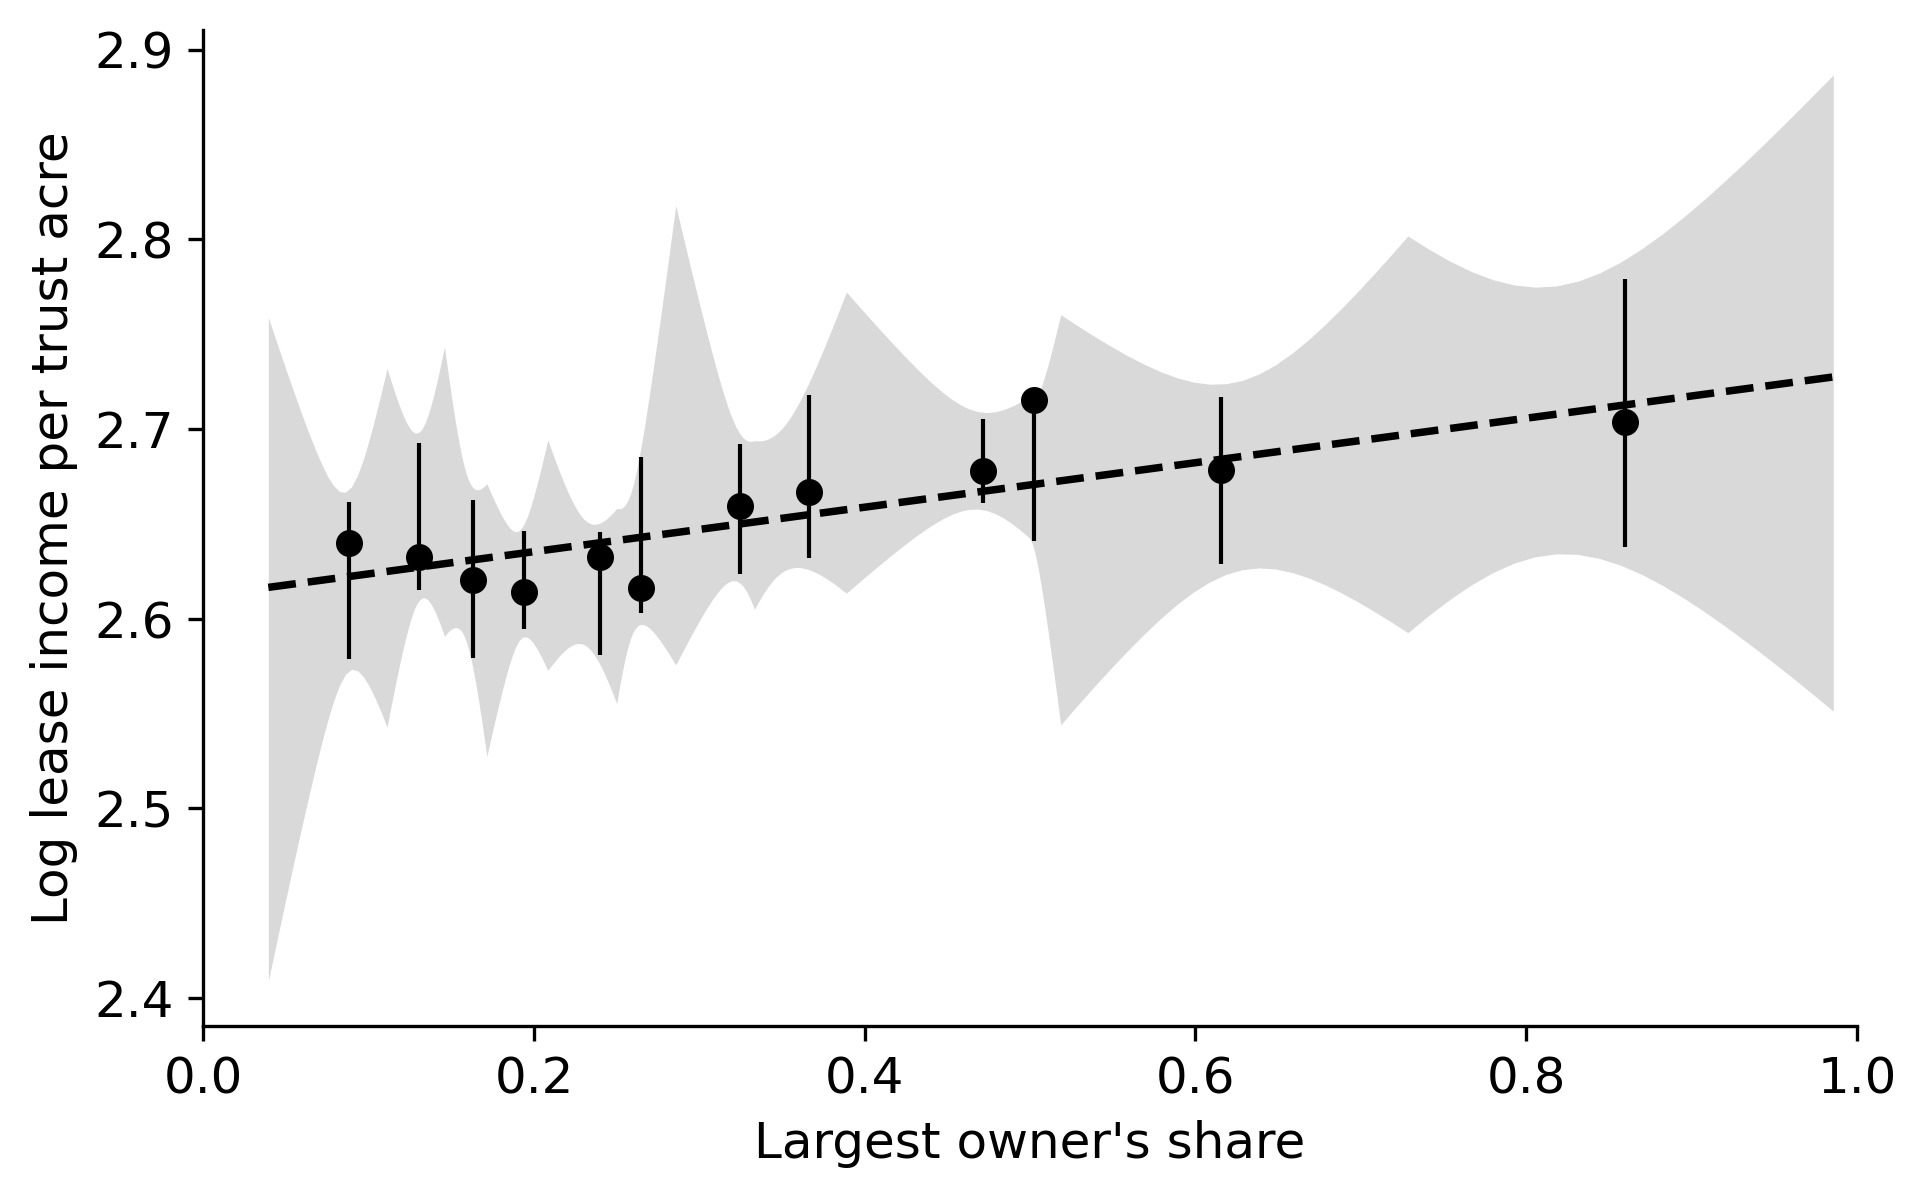
\includegraphics[width=0.78\textwidth]{max_share.png}
\begin{minipage}{0.72\linewidth}
\vspace{0.25em}
\caption*{\footnotesize Notes: The unit of observation is a tract with an agricultural lease signed between 2006 and 2010. Each point is the mean of log lease income per trust acre within a 0.05-wide bin of the largest owner's share, after partialling out reservation and lease-signing year fixed effects and the lease-level controls, with a vertical bar giving the 95 percent confidence interval for the bin mean. The solid line is a linear fit and the shaded region its 95 percent confidence band, clustered by reservation. A binscatter linearity test does not reject a linear relationship ($p=0.19$). $N=8,662$ across 45 reservations.}
\end{minipage}
\end{figure}

\begin{figure}[H]
\centering
\caption{\label{fig2} Lease Income per Trust Acre and Number of Owners}
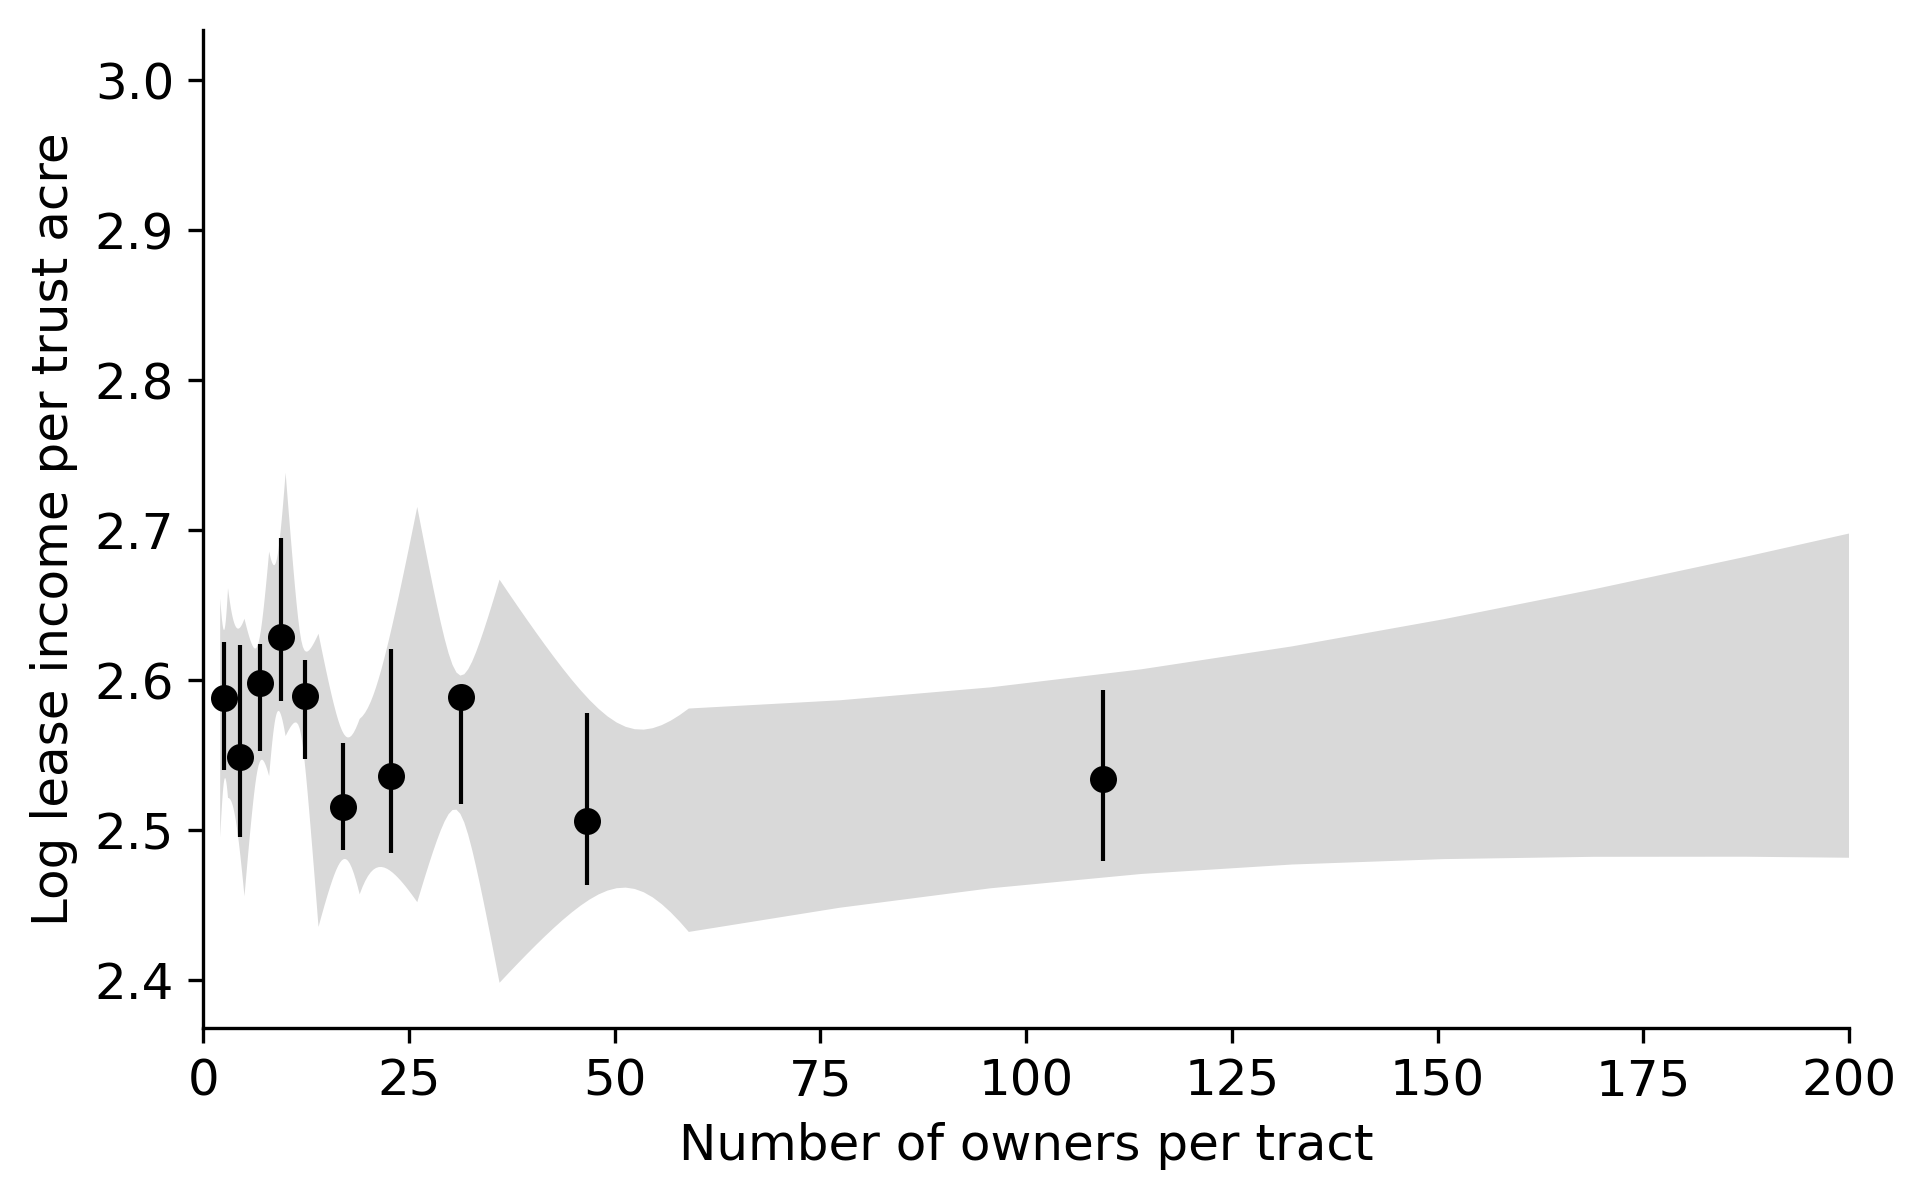
\includegraphics[width=0.78\textwidth]{owners.png}
\begin{minipage}{0.72\linewidth}
\vspace{0.25em}
\caption*{\footnotesize Notes: The unit of observation is a tract with an agricultural lease signed between 2006 and 2010, restricted to tracts with no tribal ownership. Each point is the mean of log lease income per trust acre within a bin two owners wide, after partialling out reservation and lease-signing year fixed effects and the lease-level controls, with a vertical bar giving the 95 percent confidence interval for the bin mean. The shaded region is a 95 percent confidence band that is heteroskedasticity-robust. No linear overlay is drawn, because a binscatter linearity test rejects a linear relationship ($p=0.02$). $N=5,018$ across 43 reservations.}
\end{minipage}
\end{figure}

\clearpage

\begin{table}[H]
\caption{First Stage and Reduced Form}
\label{tab:iv_firststage}
\setlength\extrarowheight{-6pt}
\estwide{table_iv_firststage_reducedform_crowex.tex}{2}{c}
\parbox{1\textwidth}{\begin{spacing}{0.8}
\small Notes: The table reports the first stage and reduced form for the main fractionation measure, $1/\sqrt{s_{\max}}$, and the corresponding Crow-included comparison. The preferred sample excludes the Crow Reservation and includes agency-administered, multi-owner, surface-resource-only agricultural leases of allotted trust land signed between 2006 and 2010, with qualifying probate orders on or after 1938. Qualifying probate orders are approved no later than the lease effective date. Specifications include reservation fixed effects, lease-signing year fixed effects, lease term, fee-simple share, and log tract acreage. Standard errors appear in parentheses and cluster at the reservation level. The effective $F$-statistic is the Montiel Olea and Pflueger statistic.
\end{spacing}}
\end{table}

\clearpage

\begin{figure}[H]
\centering
\caption{\label{fig:iv_fs_rf} First Stage and Reduced Form}
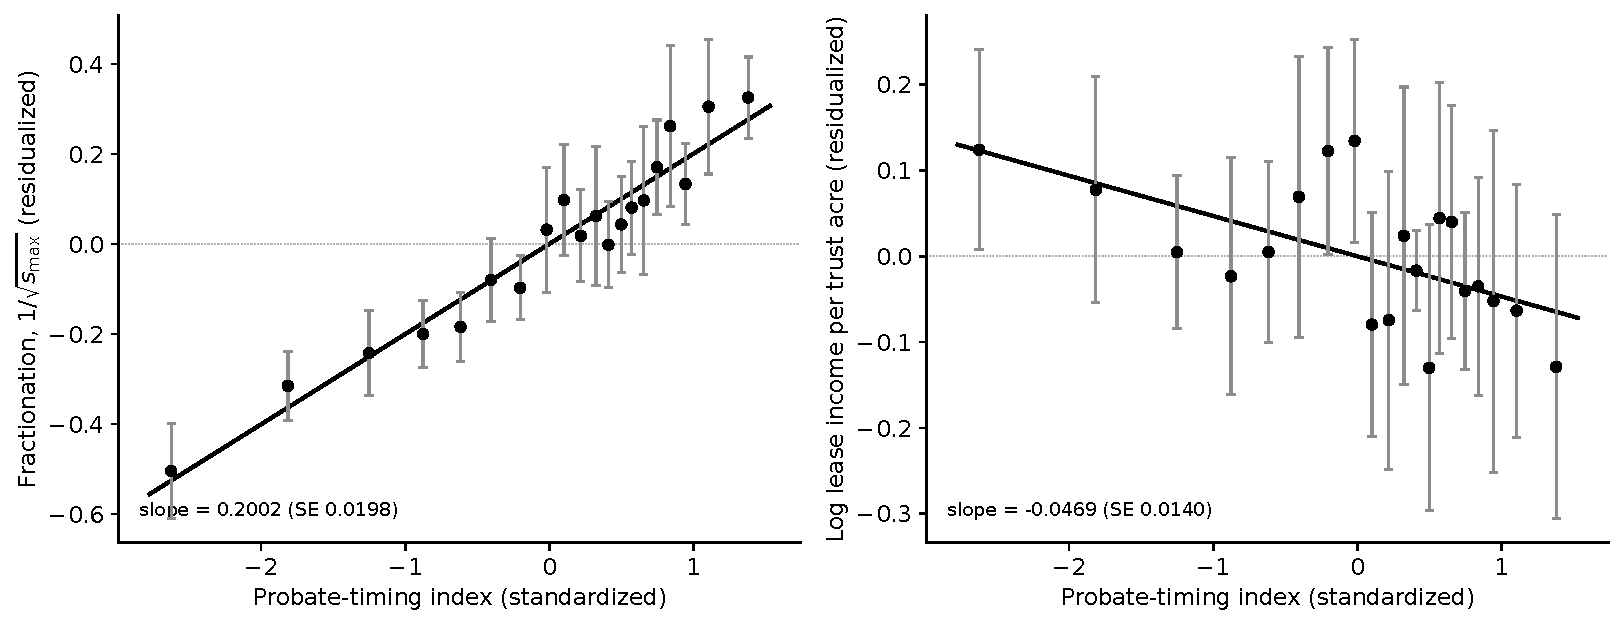
\includegraphics[width=0.98\textwidth]{fig_iv_fs_rf_nocrow_gray.pdf}
\caption*{\footnotesize Notes: Both panels use the preferred IV sample, which excludes the Crow Reservation and contains 2,211 leases across 38 reservations. The probate-timing index combines the earliest and latest qualifying probate orders using the first-stage coefficients and is standardized to mean zero and standard deviation one in the preferred IV sample. The left panel plots the first stage for the index. The right panel plots the reduced form for the index. Points are means of twenty equal-count bins of the index, with 95 percent confidence intervals clustered at the reservation level. All variables are residualized on reservation fixed effects, lease-signing year fixed effects, lease term, fee-simple share, and log tract acreage. The ratio of the reduced-form slope to the first-stage slope equals the two-stage least-squares estimate for the index specification.}
\end{figure}

\begin{table}[H]
\caption{Instrumental-Variables Estimates of the Effect of Fractionation on Lease Income per Trust Acre} \label{tab:table_iv_main}
\setlength\extrarowheight{-6pt}
\estwide{table_iv_main_crowex.tex}{4}{c}
\parbox{1\textwidth}{\begin{spacing}{0.8}
\small Notes: Each row reports a separate two-stage least-squares regression of log lease income per trust acre on the indicated ownership measure. The instruments are the earliest and latest probate orders approved no later than the lease effective date. Measures increasing in fractionation have predicted negative coefficients, while measures increasing in concentration have predicted positive coefficients. The row labeled $\ln(\text{owners})$ uses the natural logarithm of the tract owner count. The preferred sample excludes the Crow Reservation. The comparison columns include Crow. All specifications include reservation fixed effects, lease-signing year fixed effects, lease term, fee-simple share, and log tract acreage. Standard errors appear in parentheses and cluster at the reservation level. Wild-cluster bootstrap $p$-values use WRE-N, impose the null, use Rademacher weights by reservation, and use 99,999 replications. Anderson-Rubin intervals are weak-instrument-robust 95 percent confidence sets. For the main form, the conditional likelihood ratio 95 percent confidence sets are [$-0.437$, $-0.067$] in the preferred sample and [$-0.415$, 0.003] in the Crow-included comparison. The effective $F$-statistic reported at the bottom refers to the main $1/\sqrt{s_{\max}}$ row. Row-specific first-stage diagnostics for the count-based alternatives appear in Table~\ref{tab:count_iv_robustness}. The effective $F$-statistic is the Montiel Olea and Pflueger statistic. Over-identification $p$-values are Sargan tests and do not establish instrument validity.
\end{spacing}}
\end{table}

\begin{table}[H]
\caption{Instrumental-Variables Robustness}
\label{tab:table_iv_robust}
\scriptsize
\setlength\extrarowheight{-6pt}
\estwide{table_iv_robust_crowex_short.tex}{6}{c}
\parbox{1\textwidth}{\begin{spacing}{0.8}
\small Notes: Each row reports a two-stage least-squares estimate of log lease income per trust acre on $1/\sqrt{s_{\max}}$, except for rows that name another concentration measure. The instruments are the earliest and latest probate orders approved no later than the lease effective date. The table reports the preferred Crow-excluded sample and the Crow-included comparison. Specifications include reservation fixed effects, lease-signing year fixed effects, lease term, fee-simple share, and log tract acreage unless the row states otherwise. Standard errors appear in parentheses and cluster at the reservation level. Wild-cluster bootstrap $p$-values use 99,999 replications. Anderson-Rubin intervals are weak-instrument-robust 95 percent confidence sets.
\end{spacing}}
\normalsize
\end{table}

\begin{figure}[H]
\centering
\caption{\label{fig:iv_spec_curve} Instrumental-Variables Estimates Across Specifications}
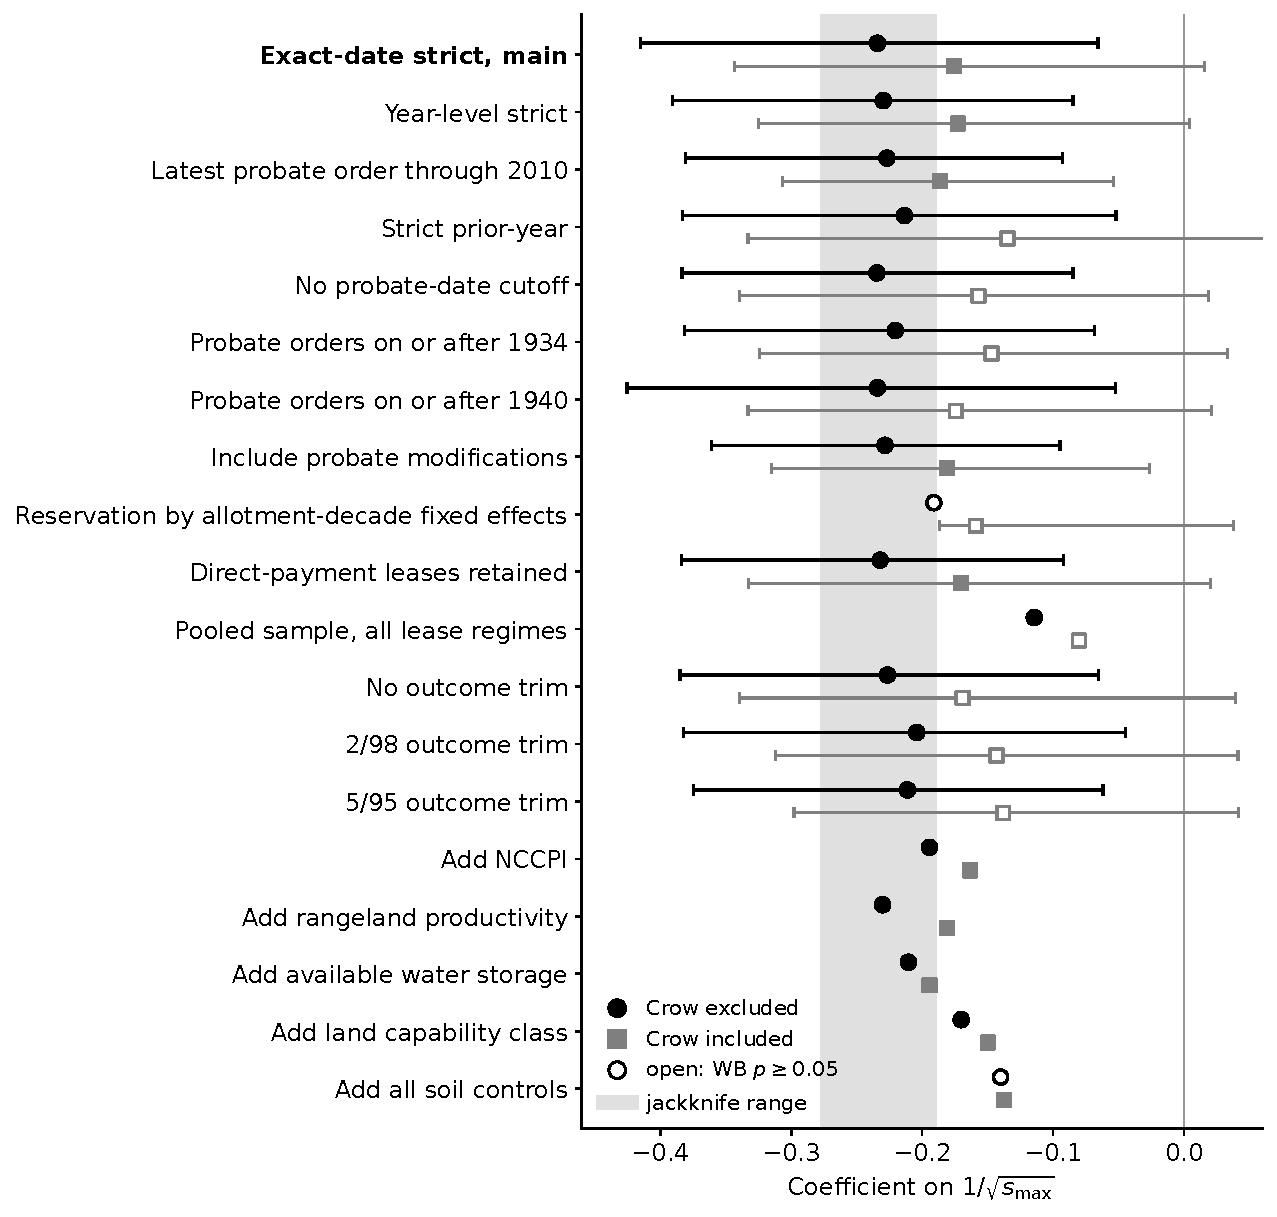
\includegraphics[width=0.96\textwidth]{fig_spec_curve_panelA.pdf}
\begin{minipage}{0.92\linewidth}
\vspace{0.35em}
{\scriptsize \emph{Notes:} This figure reports two-stage least-squares estimates of the effect of
ownership fractionation on log annual lease income per trust acre for the main fractionation
measure, $1/\sqrt{s_{\max}}$, across instrument constructions, probate windows, sample
restrictions, outcome trims, and soil controls. Crow-excluded estimates use the preferred sample
(circles). Crow-included estimates repeat the same specifications with the Crow Reservation included
(squares). Horizontal bars are Anderson--Rubin 95 percent confidence sets, shown where available.
Bars are omitted for the soil-control variants, the pooled sample, and the
reservation-by-allotment-decade specification, where an Anderson--Rubin set was not computed.
Filled markers denote wild-cluster bootstrap $p$-values below $0.05$. Open markers denote
$p$-values at or above $0.05$. The shaded band shows the leave-one-reservation-out coefficient
range in the preferred sample. The figure summarizes robustness and does not introduce a separate
identification design.\par}
\end{minipage}
\end{figure}

\clearpage

\begin{table}[H]
\caption{Tribal Largest Ownership and Lease Income per Trust Acre}
\centering
\label{tab:table4}
\setlength\extrarowheight{-6pt}
\estwide{table4.tex}{4}{c}
\parbox{1\textwidth}{\begin{spacing}{0.8}
\small Notes: This table reports ordinary least-squares regressions of log annual lease income per trust acre on an indicator for the tribe being the largest owner of the tract. The sample includes agricultural leases of allotted trust land signed between 2006 and 2010. Columns 1 through 3 use the full constructed sample. Column 4 uses the multi-owner sample. All columns include reservation fixed effects and lease-signing year fixed effects. Lease controls are lease term, resource-type indicators, and log tract acreage. Standard errors appear in parentheses and cluster at the reservation level. Wild-cluster bootstrap $p$-values are reported in the table and use Rademacher weights by reservation with the null imposed. These estimates are descriptive associations and do not identify a causal effect of tribal ownership.
\end{spacing}}
\end{table}

\begin{table}[H]
\caption{Direct Payment and Lease Income per Trust Acre}
\centering
\label{tab:table8}
\setlength\extrarowheight{-6pt}
\estwide{tableDir.tex}{4}{c}
\parbox{1\textwidth}{\begin{spacing}{0.8}
\small Notes: This table reports ordinary least-squares regressions of log annual lease income per trust acre on direct-payment measures. Direct payment is a proxy for owner involvement in the lease. Columns 1, 3, and 4 use the directly paid ownership share. Column 2 uses an indicator for a direct-payment lease. The sample includes agricultural leases of allotted trust land signed between 2006 and 2010. All specifications include reservation fixed effects, lease-signing year fixed effects, lease term, fee-simple share, and log tract acreage. Standard errors appear in parentheses and cluster at the reservation level. Wild-cluster bootstrap $p$-values are reported in the table and use Rademacher weights by reservation with the null imposed. These estimates are descriptive associations and do not identify a causal effect of direct payment.
\end{spacing}}
\end{table}

\begin{figure}[H]
\centering
\caption{\label{fig3} Lease Income per Trust Acre and Tribal Ownership Share}
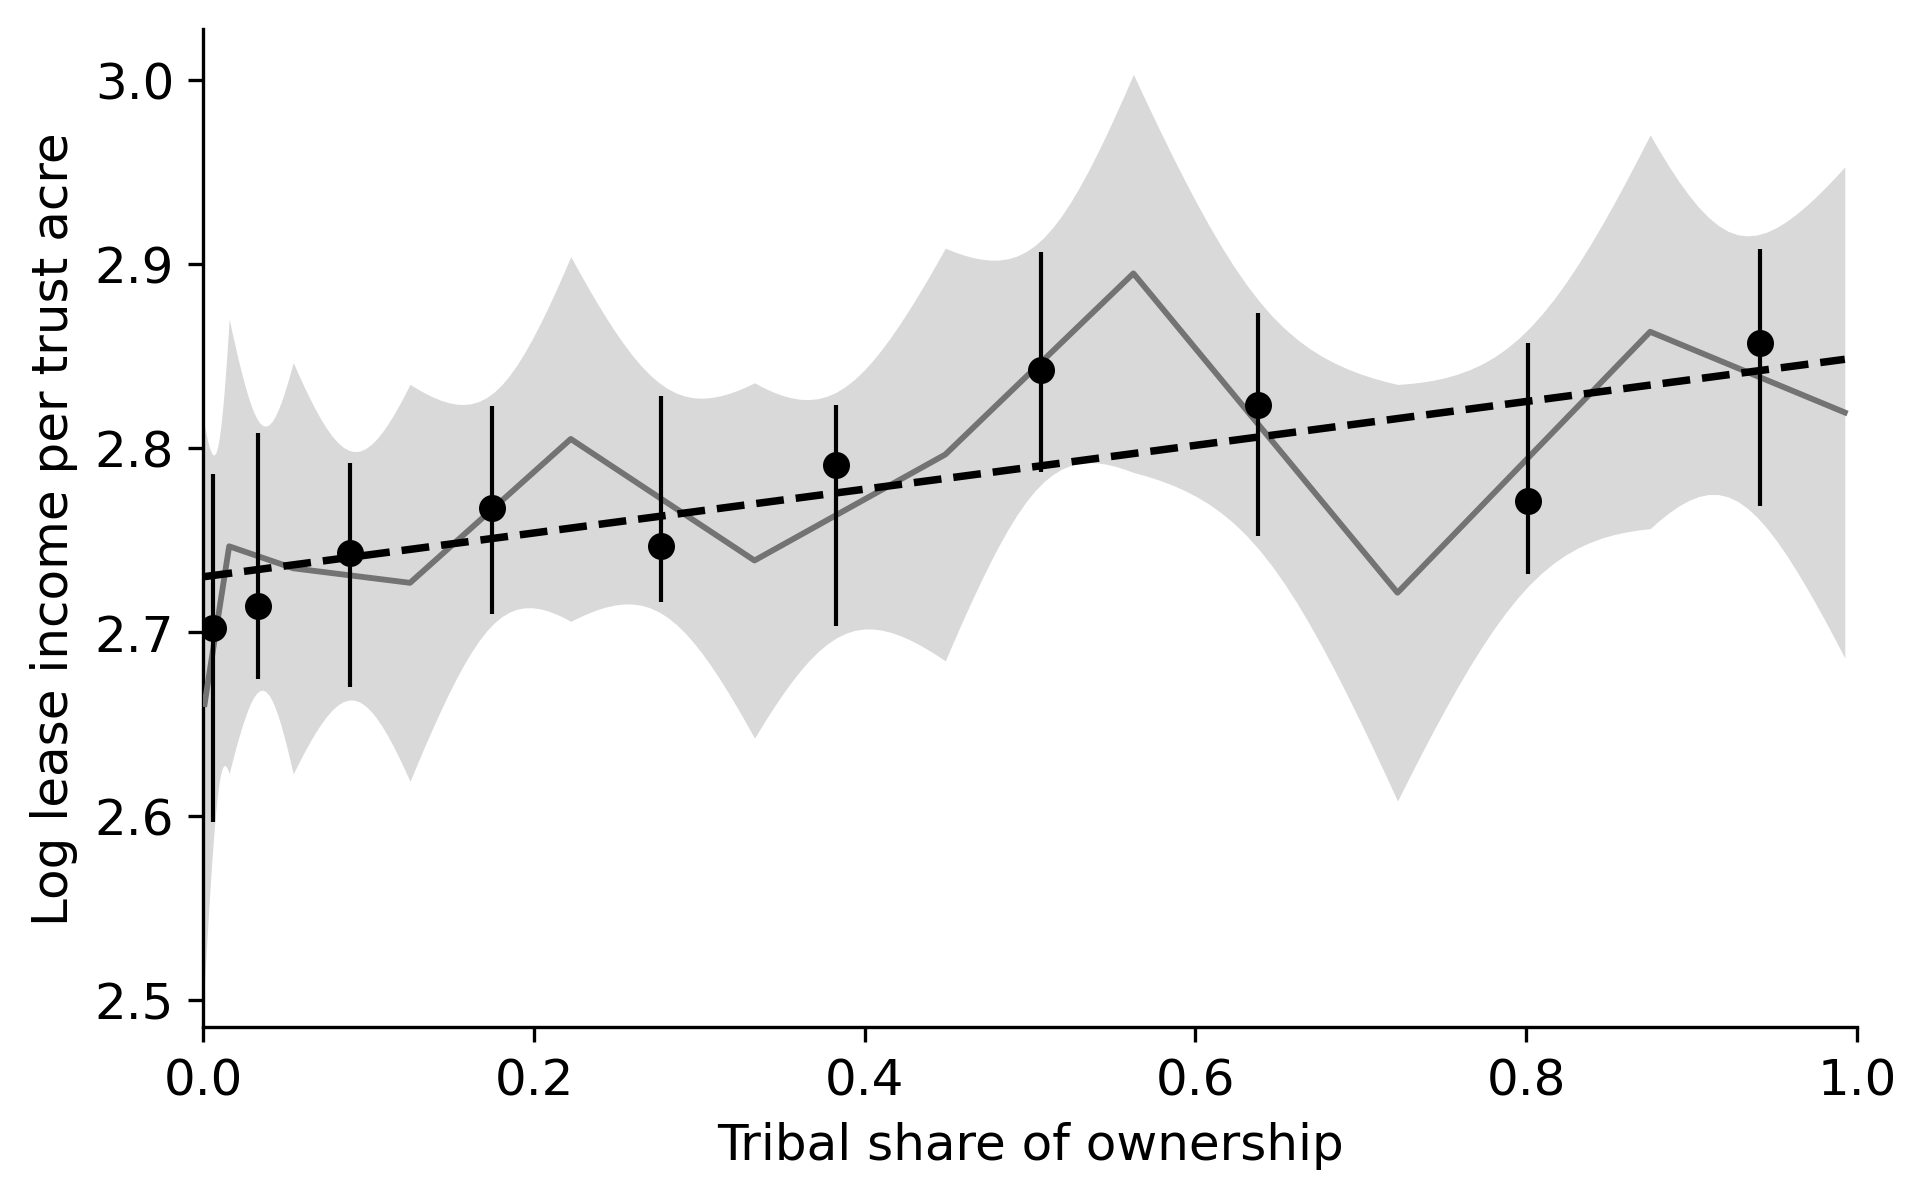
\includegraphics[width=0.78\textwidth]{tribe_interest.png}
\begin{minipage}{0.72\linewidth}
\vspace{0.25em}
\caption*{\footnotesize Notes: The unit of observation is a tract with an agricultural lease signed between 2006 and 2010, restricted to tracts with a positive tribal ownership share. Each point is the mean of log lease income per trust acre within a 0.05-wide bin of the tribal share, after partialling out reservation and lease-signing year fixed effects and the lease-level controls, with a vertical bar giving the 95 percent confidence interval for the bin mean. The solid line is a linear fit and the shaded region a 95 percent confidence band that is heteroskedasticity-robust. A binscatter linearity test does not reject linearity at conventional levels ($p=0.07$). $N=3,643$ across 40 reservations.}
\end{minipage}
\end{figure}

\begin{figure}[H]
\centering
\caption{\label{fig4} Agency Pay and Direct Pay by Number of Owners per Tract}
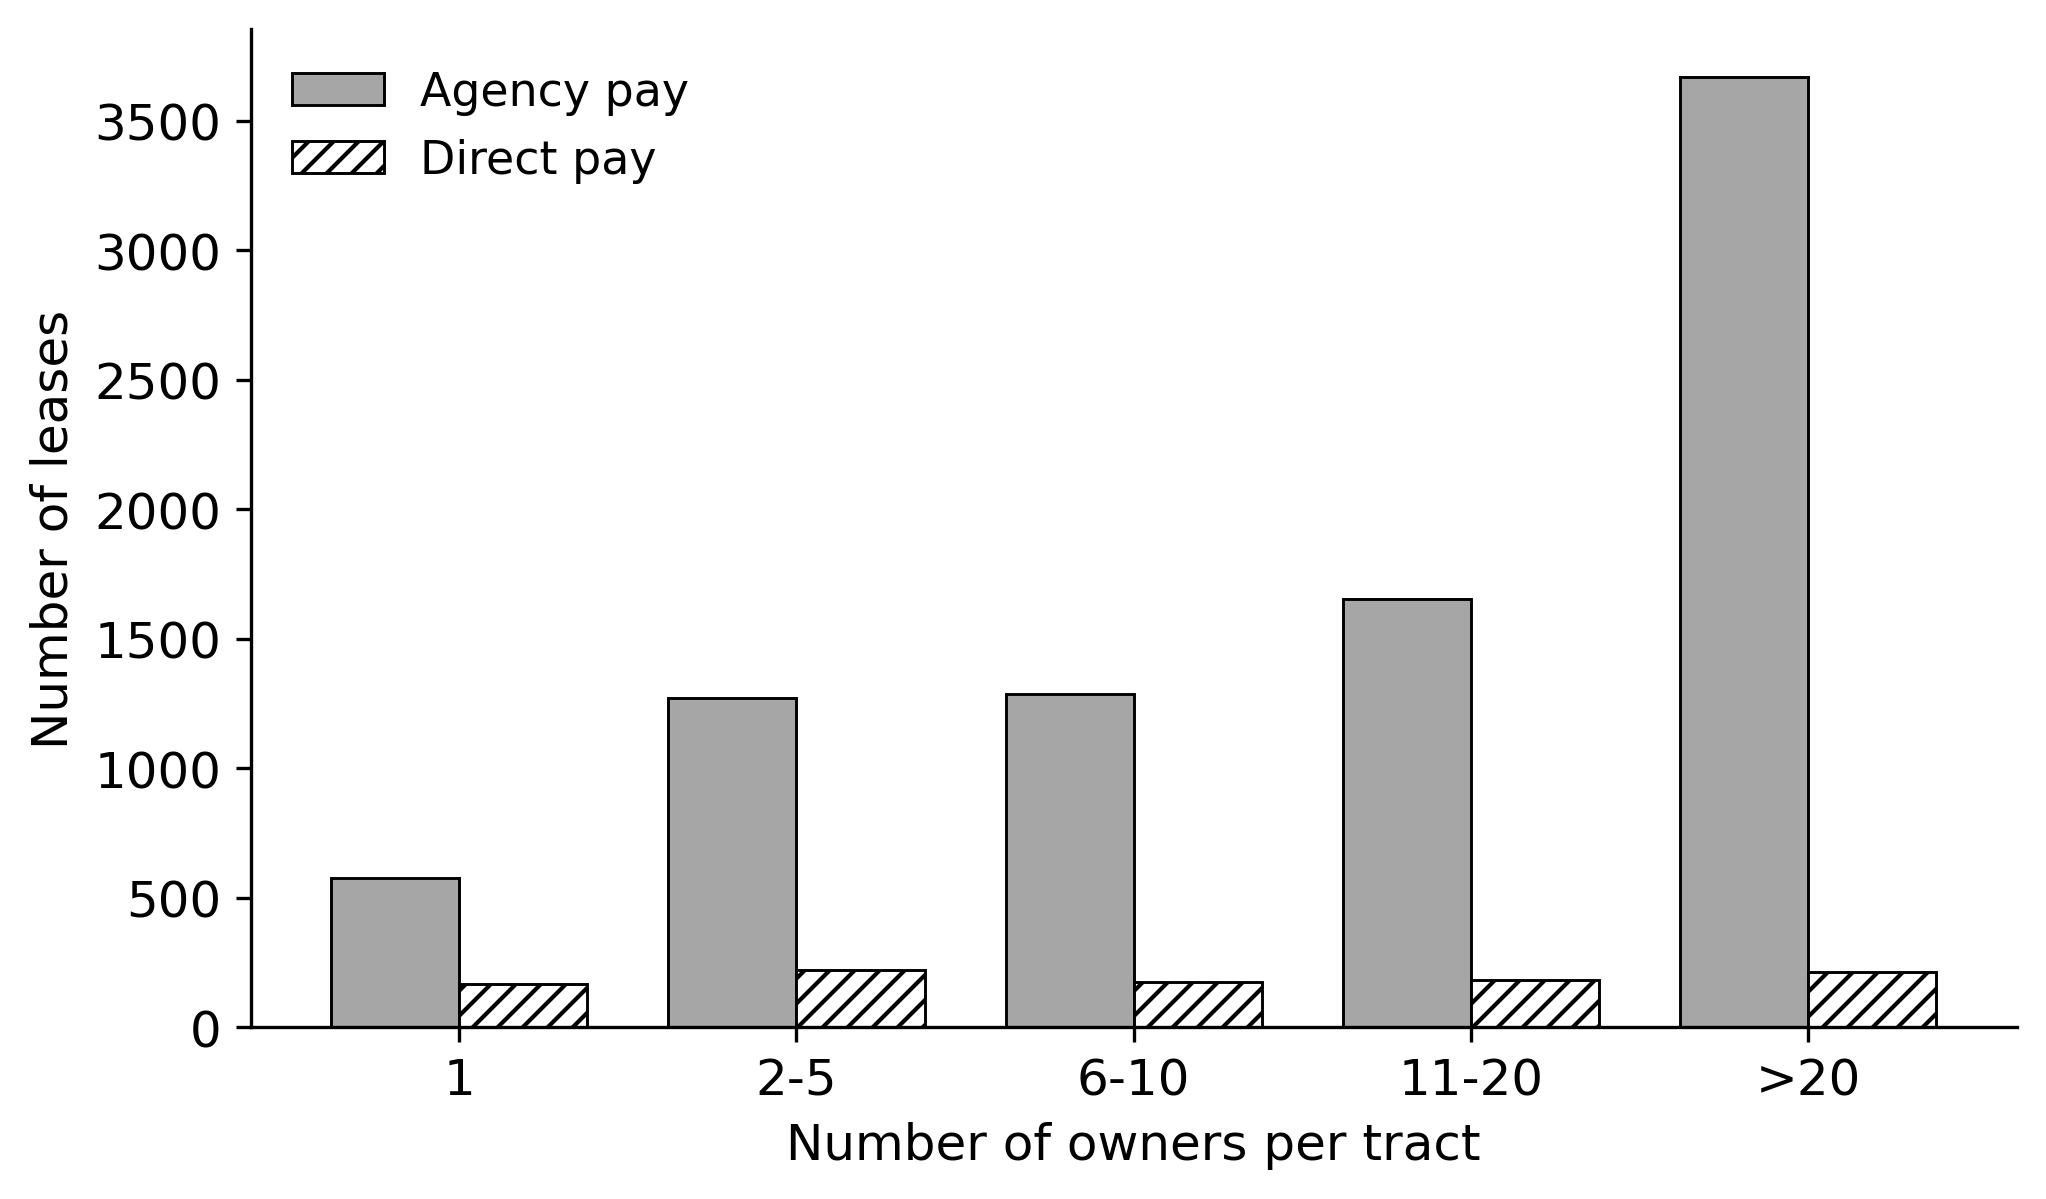
\includegraphics[width=0.78\textwidth]{direct.png}
\begin{minipage}{0.72\linewidth}
\vspace{1mm}
\caption*{\footnotesize Notes: The unit of observation is an agricultural lease signed between 2006 and 2010. Bars give the number of leases in each owner count category, shown separately for leases paid through the agency and leases paid directly to the owners. $N=9{,}409$.}
\end{minipage}
\end{figure}

\begin{table}[H]
\caption{Calibration Inputs and Implied Monitoring Gap}
\label{tab:calibration_crowex}
\setlength\extrarowheight{-6pt}
\estwide{table_calibration_crowex.tex}{2}{c}
\parbox{1\textwidth}{\begin{spacing}{0.8}
\small Notes: The table reports the descriptive model-based calibration from the levels regression of lease income per trust acre on $1/\sqrt{s_{\max}}$, estimated without controls or fixed effects. The Crow-excluded column uses the broad calibration sample of 8,387 leases and is reported as the main descriptive calibration because the preferred institutional population excludes Crow. It is not the preferred IV sample. The Crow-included column is reported for comparison. Dollars are 2010 dollars per trust acre unless otherwise stated. The calibration is not the causal IV estimate. IV-based scale translations reported in the text imply larger output gaps under the preferred probate-timing design.
\end{spacing}}
\end{table}

\begin{figure}[H]
\centering
\caption{\label{fig6} Simulated Output Gap}
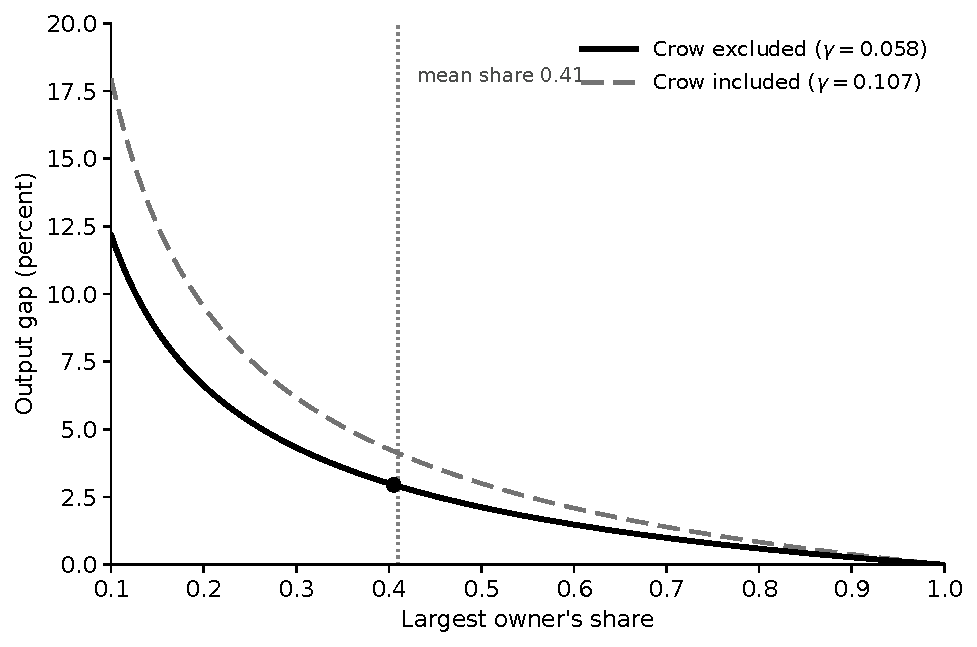
\includegraphics[width=0.72\textwidth]{fig_output_gap_crowex.pdf}
\begin{minipage}{0.82\linewidth}
\vspace{0.25em}
% beneath the figure in main.tex. Keep this note in LaTeX, not inside the image.
{\footnotesize \emph{Notes:} This figure plots the model-implied output gap, $(R^{*}-R)/R$,
against the largest owner's share, where $R$ is realized lease income per trust acre at a given
share and $R^{*}$ is income under the constrained efficient benchmark. The solid line is the Crow-excluded descriptive calibration ($\gamma=0.058$). The dashed line is the Crow-included comparison
($\gamma=0.107$). The vertical dotted line marks the mean largest owner's share in the
Crow-excluded calibration sample, $0.41$, where the implied gap is about $3.0$ percent of lease
income. The figure is a model-based calibration from the descriptive levels equation. It is not a second source of causal identification and does not display the IV-based scale translations discussed in the text.\par}
\end{minipage}
\end{figure}


\clearpage
\section*{Appendix A\centering} \label{AppendixA}
\setcounter{figure}{0}
\renewcommand{\thefigure}{A\arabic{figure}}
\renewcommand{\theHfigure}{A\arabic{figure}}
\setcounter{table}{0}
\renewcommand{\thetable}{A\arabic{table}}
\renewcommand{\theHtable}{A\arabic{table}}




\subsection*{The Organized-Owner Extension}
\setcounter{equation}{0}
\renewcommand{\theequation}{A\arabic{equation}}
\renewcommand{\theHequation}{A\arabic{equation}}

An organized owner is an owner whose organizational form or formal access to the agency lowers the unit cost of monitoring. In the application, a tribal owner is the leading example. This appendix extends the theoretical model by allowing owners to differ in monitoring costs as well as in output shares. Section~\ref{Theory} shows that, with common monitoring costs, the largest ownership share determines which owner contributes monitoring in equilibrium. With unequal costs, the relevant object is the cost-adjusted ownership share.

We consider two owners who may contribute monitoring: an organized owner $g$ and an individual owner $I$, the individual with the largest ownership share. Other individual owners have weakly smaller shares and the same unit monitoring cost as owner $I$, so none has a larger cost-adjusted ownership share than $I$. It is therefore sufficient to compare owner $g$ with owner $I$. Aggregate monitoring is $M=m_g+m_I$.

Normalize the organized owner's unit cost of monitoring to 1, and let owner $I$'s unit cost be $c_I\geq 1$. The organized owner's payoff is $\pi_g=s_gR-m_g$, where $s_g$ is its output share and $m_g$ is its monitoring contribution. Owner $I$'s payoff is $\pi_I=s_I R-c_I m_I$, where $s_I$ is that owner's output share and $m_I$ is that owner's monitoring contribution.

For any owner $k$ with output share $s_k$ and unit monitoring cost $c_k$, the monitoring level it would choose if the other owner contributed zero is $\sqrt{R_l\gamma}\sqrt{s_k/c_k}-\gamma$. The object $s_k/c_k$ is the cost-adjusted ownership share. The best response for owner $I$ is
\begin{equation} \label{(11)}
    m_I = \max\left\{\sqrt{R_l \gamma}\sqrt{\frac{s_I}{c_I}} -\gamma-m_g,0\right\},
\end{equation}
\noindent
and the best response for the organized owner is
\begin{equation} \label{(12)}
    m_g = \max\left\{\sqrt{R_l \gamma}\sqrt{s_g}-\gamma-m_I,0\right\}.
\end{equation}

The equilibrium depends on the comparison between $s_g$ and $s_I/c_I$. If $s_g>s_I/c_I$, the organized owner has the larger cost-adjusted ownership share. In equilibrium, the organized owner contributes all monitoring and owner $I$ contributes zero. Aggregate monitoring is
\begin{equation} \label{(13)}
   M=\sqrt{R_l\gamma}\sqrt{s_g}-\gamma,
\end{equation}
\noindent
and output is
\begin{equation} \label{(14)}
   R=R_l -\sqrt{R_l\gamma} \left(\frac{1}{\sqrt{s_g}}\right).
\end{equation}
The constrained efficient benchmark remains $M^* = \sqrt{R_l \gamma} - \gamma$. Because the organized owner has the lowest unit monitoring cost, a planner assigns all monitoring to that owner. The output gap is therefore
\begin{equation} \label{(15)}
    R^*-R = -\sqrt{R_l\gamma}+\sqrt{R_l\gamma}\left(\frac{1}{\sqrt{s_g}}\right).
\end{equation}

If $s_I/c_I>s_g$, owner $I$ has the larger cost-adjusted ownership share. In equilibrium, owner $I$ contributes all monitoring and the organized owner contributes zero. Aggregate monitoring is
\begin{equation} \label{(16)}
   M=\sqrt{R_l\gamma}\sqrt{\frac{s_I}{c_I}} -\gamma,
\end{equation}
\noindent
output is
\begin{equation} \label{(17)}
   R=R_l -\sqrt{R_l\gamma}\sqrt{\frac{c_I}{s_I}},
\end{equation}
\noindent
and the output gap is
\begin{equation} \label{(18)}
   R^*-R = -\sqrt{R_l\gamma}+\sqrt{R_l\gamma}\sqrt{\frac{c_I}{s_I}}.
\end{equation}

If $s_g=s_I/c_I$, the two owners have the same cost-adjusted ownership share. The equilibrium allocation of monitoring between them is not unique. Any nonnegative split between $m_g$ and $m_I$ that delivers total monitoring
\begin{equation} \label{(19)}
   M=\sqrt{R_l\gamma}\sqrt{s_g}-\gamma = \sqrt{R_l\gamma}\sqrt{\frac{s_I}{c_I}} -\gamma
\end{equation}
\noindent
is an equilibrium and yields the same output.

The extension preserves the public-goods logic of the main model. With equal costs, the largest ownership share determines which owner contributes monitoring in equilibrium. With unequal costs, the cost-adjusted ownership share determines which owner contributes monitoring. Monitoring and output rise with that owner's ownership share and fall with that owner's unit monitoring cost. A lower monitoring cost can make an organized owner contribute all monitoring even when its ownership share is below that of the largest individual owner.


\subsection*{Distributions of Key Variables}

Figures \ref{figA1}, \ref{figA2}, \ref{figA3}, and \ref{figA4} visualize some of the variables described in Table \ref{tab:table1}. Figure \ref{figA1} shows the frequency distribution of lease income. Figure \ref{figA2} shows the distribution of the number of owners per tract. Figure \ref{figA3} shows the frequency distribution of the largest ownership share for each tract. This distribution shows 25, 33, and 50 percent peaks, about 800 observations in these three categories. For about 25 percent of all tracts, the largest ownership share is less than 20 percent. The histogram in Figure \ref{figA4} shows the subsample of tracts in which the tribe shares ownership. Of these tracts, 1,000 have less than a ten percent tribal ownership share. The tribal ownership shares above ten percent have a roughly uniform distribution, except when tribes have 50 percent ownership in the land.
\vspace{2mm}

\begin{figure}[H]
\centering
\caption{\label{figA1} Frequency Distribution of Lease Income per Trust Acre (in 2010 dollars)}
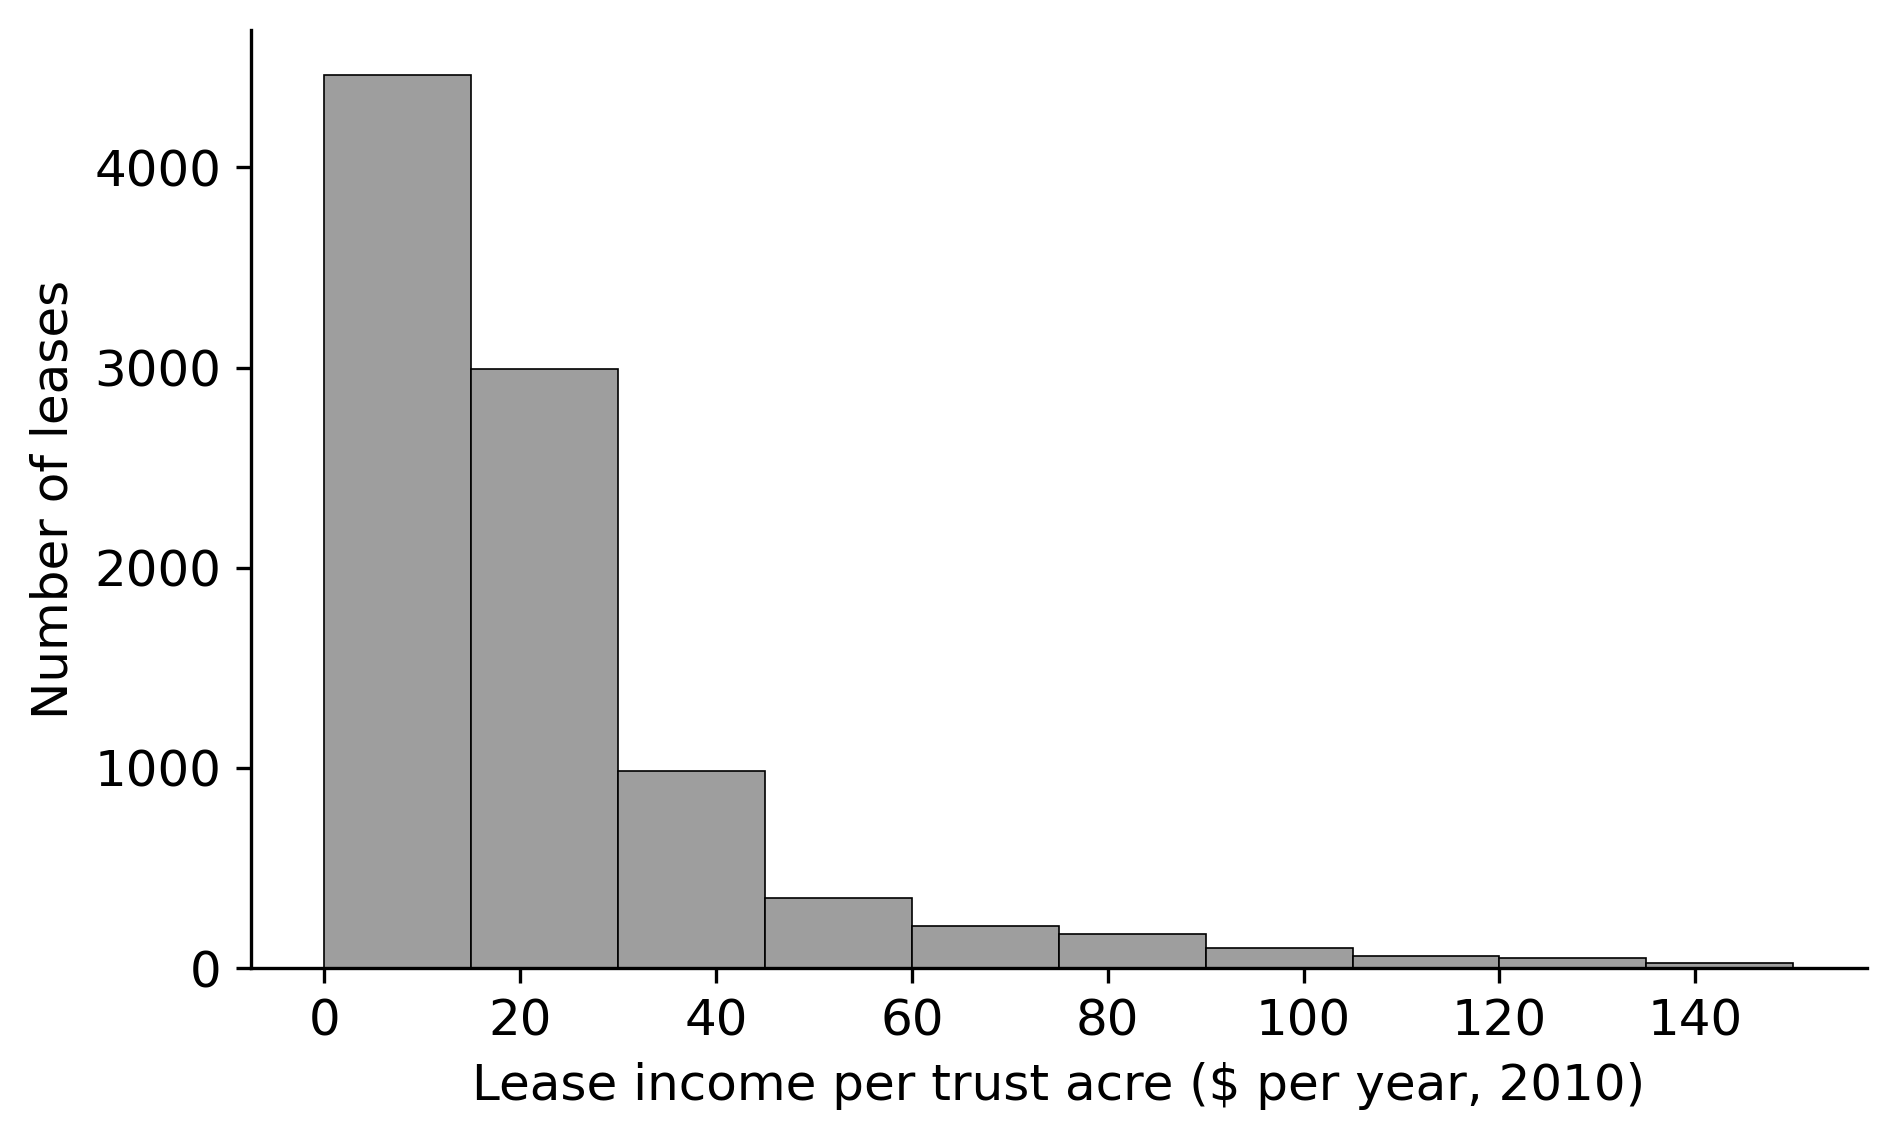
\includegraphics[width=0.78\textwidth]{inc_distr.png}
\begin{minipage}{0.70\linewidth}
\begin{flushleft}
\vspace{0.25em}
\caption*{\footnotesize Notes: The unit of observation is an agricultural lease signed between 2006 and 2010. The width of the bins is \$15. $N=9,409$.}
\end{flushleft}
\end{minipage}
\end{figure}


\begin{figure}[H]
\centering
\caption{\label{figA2} Frequency Distribution of the Number of Owners per Tract}
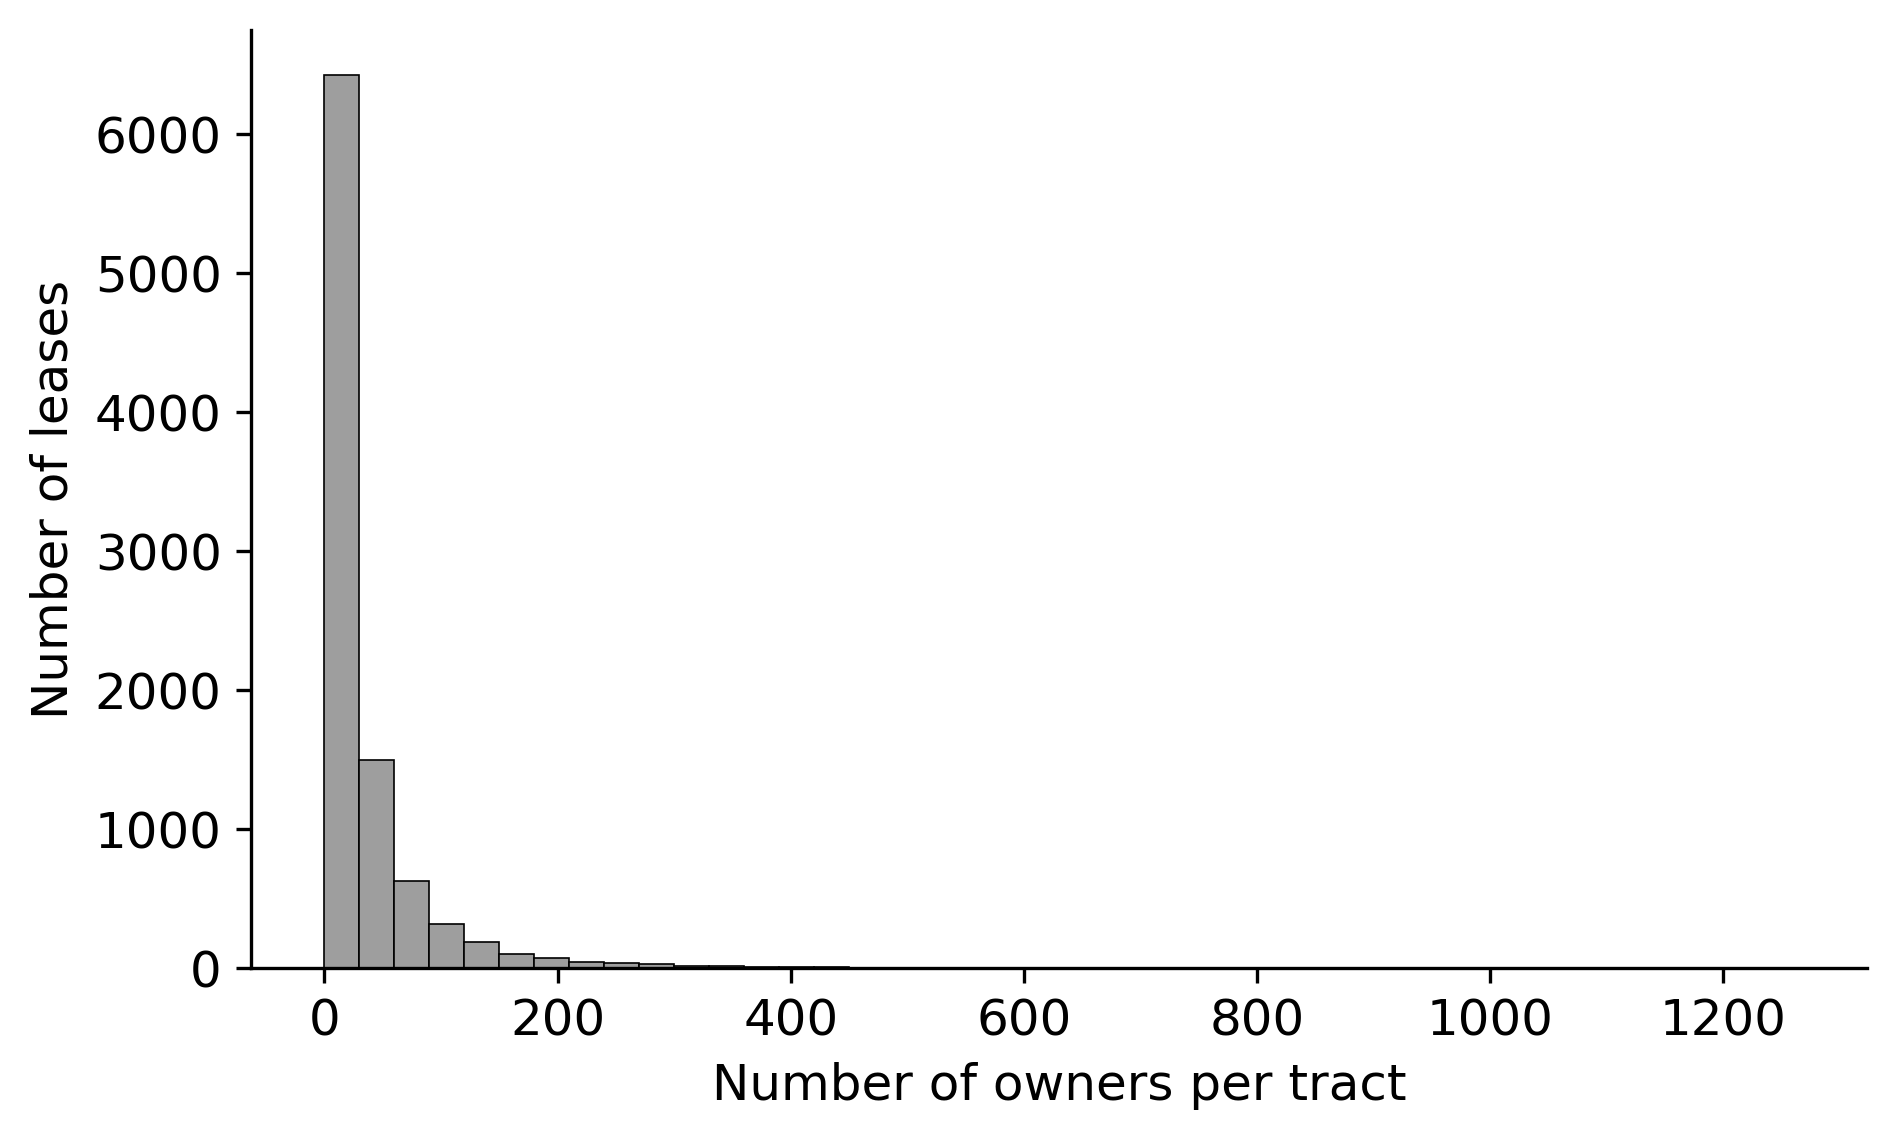
\includegraphics[width=0.78\textwidth]{owners_distr.png}
\begin{minipage}{0.70\linewidth}
\begin{flushleft}
\vspace{0.25em}
\caption*{\footnotesize Notes: The unit of observation is an agricultural lease signed between 2006 and 2010. The width of the bins is 30 owners. $N=9,409$.}
\end{flushleft}
\end{minipage}
\end{figure}


\begin{figure}[H]
\centering
\caption{\label{figA3} Frequency Distribution of the Largest Ownership Share}
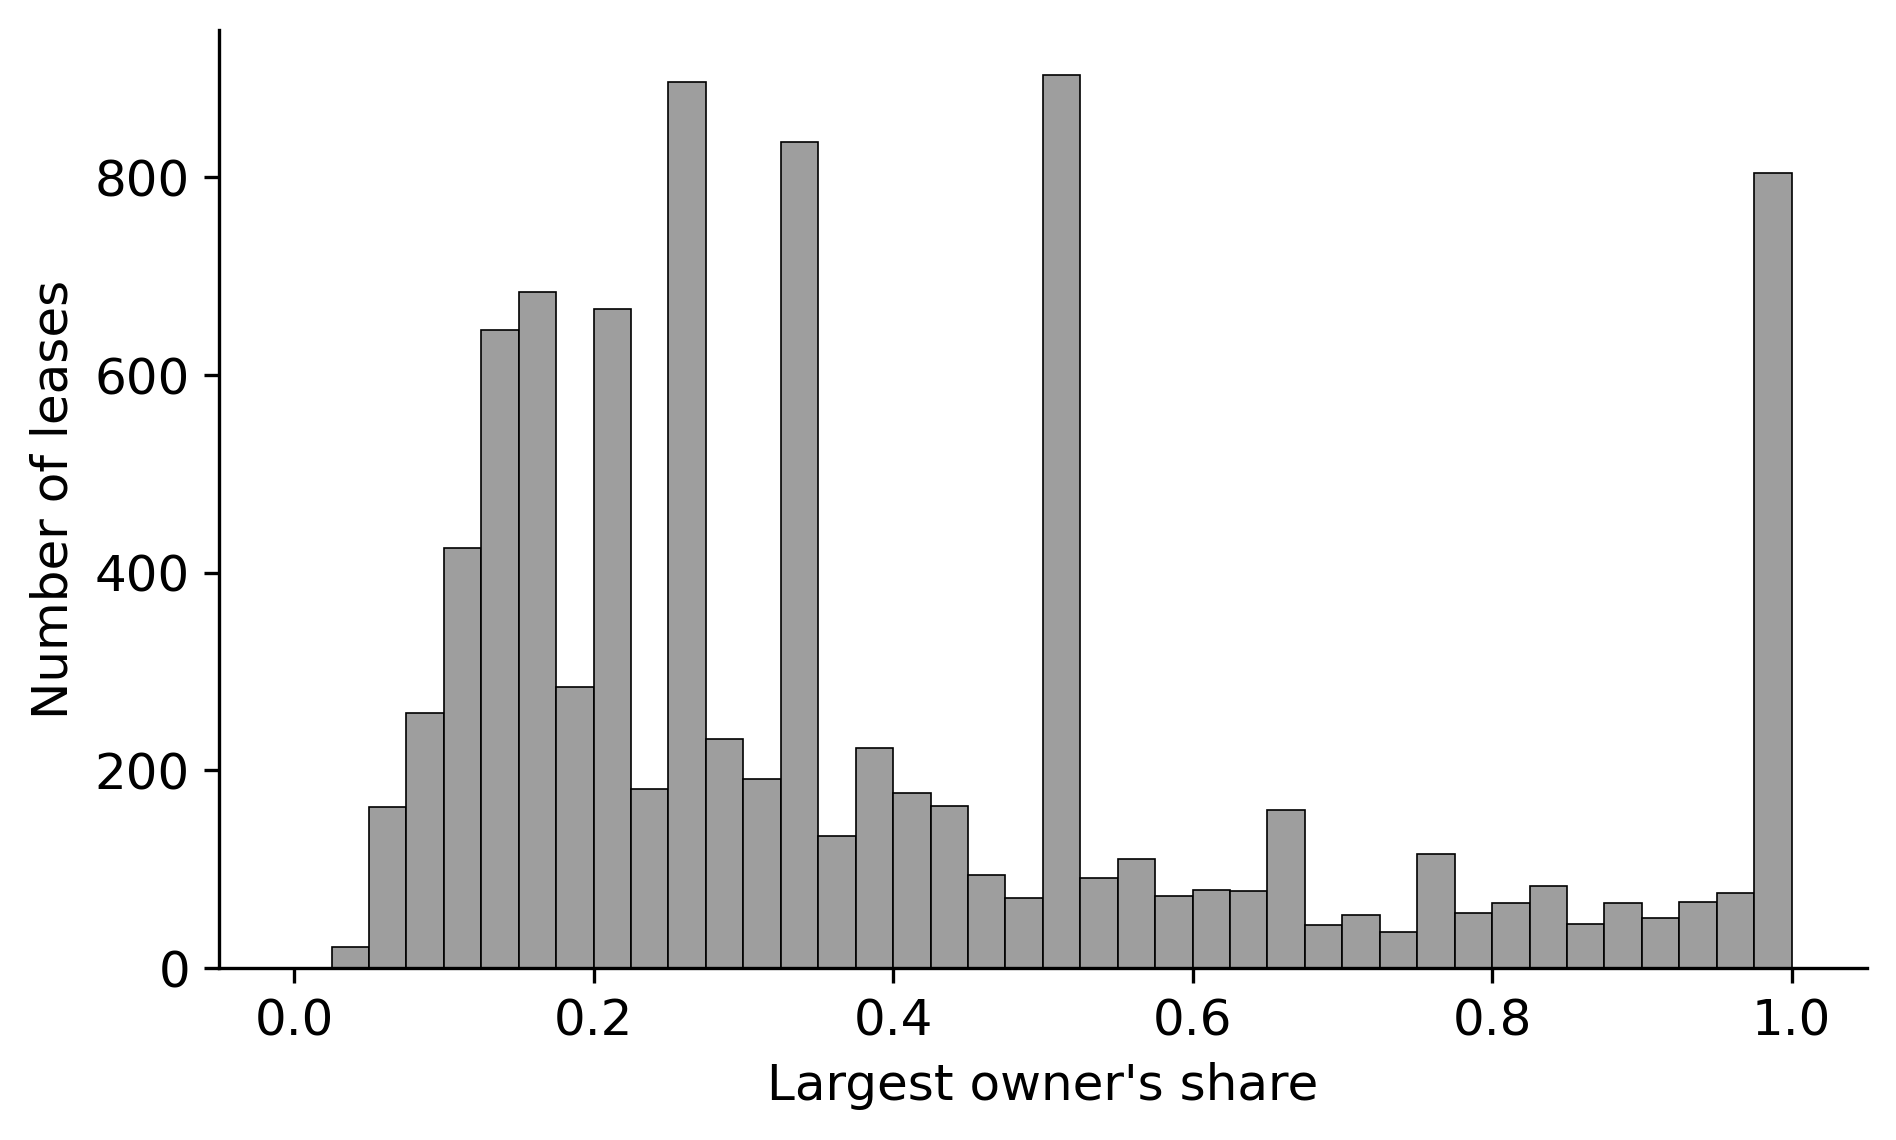
\includegraphics[width=0.78\textwidth]{max_distr.png}
\begin{minipage}{0.70\linewidth}
\begin{flushleft}
\vspace{0.25em}
\caption*{\footnotesize Notes: The unit of observation is a tract with an agricultural lease signed between 2006 and 2010. The width of the bins is 0.025 ownership share. $N=9,409$.}
\end{flushleft}
\end{minipage}
\end{figure}


\begin{figure}[H]
\centering
\caption{\label{figA4} Frequency Distribution of the Tribal Ownership Share \\ on Leases with Tribal Ownership}
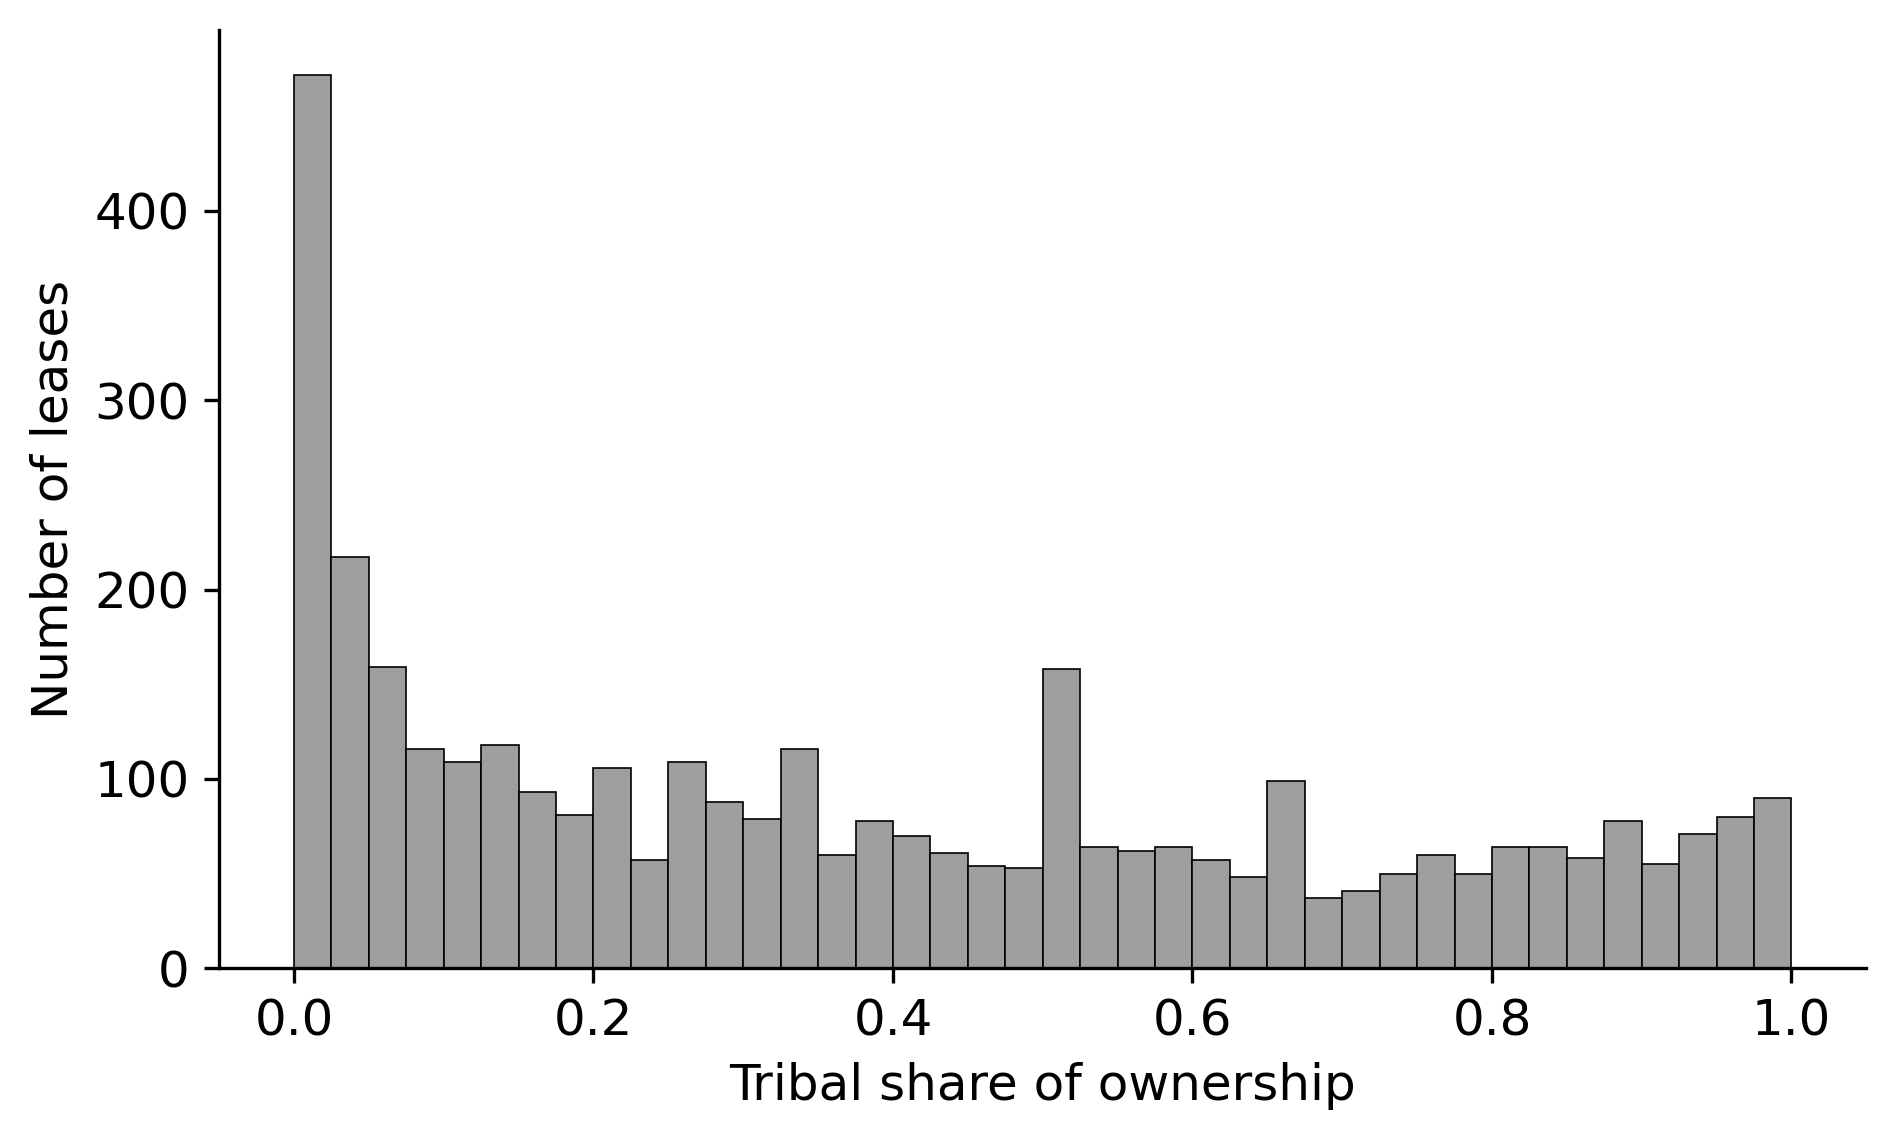
\includegraphics[width=0.78\textwidth]{tribeint_distr.png}
\begin{minipage}{0.71\linewidth}
\begin{flushleft}
\vspace{0.25em}
\caption*{\footnotesize Notes: The unit of observation is a tract with an agricultural lease signed between 2006 and 2010. The width of the bins is 0.025 ownership share. Data include only leases with a positive tribal ownership share in the leased tract. $N=3,646$.}
\end{flushleft}
\end{minipage}
\end{figure}


\clearpage


\begin{table}[H]
\caption{Lease Income per Trust Acre and Tribal Share, with the Largest-Owner Interaction}
\centering
\label{tab:table5}
\scriptsize
\setlength\extrarowheight{-6pt}
\estfit{table5.tex}{6}{c}
\setlength\extrarowheight{-6pt}
\estfit{tableB5short.tex}{6}{c}
\vspace{-1mm}
\parbox{1\textwidth}{
\begin{spacing}{0.8}
Notes: The outcome is the log of annual lease income per trust acre. Columns 1 to 3 enter the tribal ownership share alone under progressively richer controls. Columns 4 to 6 add an indicator for the tribe being the largest owner and its interaction with the tribal share. Standard errors clustered at the reservation level appear in parentheses, and wild-cluster bootstrap p-values appear in square brackets. Data in Panel B exclude leases with one owner. The specifications in Panel B include the same controls as in Panel A.
\end{spacing}
}
\normalsize
\end{table}


The remaining tables examine the tribal-ownership association under alternative codings and functional forms. Table~\ref{tab:table_play1} replaces the largest-owner indicator with an indicator for any tribal interest in the tract. Its coefficient is small and not distinguishable from zero, so the income difference in Table~\ref{tab:table4} reflects the tribe's being the largest owner rather than its mere presence. Table~\ref{tab:table_play4} enters the tribal share in the inverse-square-root form implied by the model and, alongside it, as a linear term, on the subsample of tracts with a positive tribal share. The linear association is positive and significant while the theory-implied form is not, so the tribal-share gradient is present but does not take the sharp shape the model predicts for the largest owner's share.

\begin{table}[H]
\caption{Lease Income per Trust Acre and the Presence of Tribal Ownership} \label{tab:table_play1}
\setlength\extrarowheight{-6pt}
\estwide{play_tribe_dum.tex}{3}{c}
	
\end{table}


\begin{table}[H]
\caption{Lease Income per Trust Acre and Tribal Share, Theory-Implied and Linear Forms} \label{tab:table_play4}
\scriptsize
\setlength\extrarowheight{-6pt}
\estfit{play_tribe4.tex}{6}{c}
\normalsize
\end{table}



\subsection*{Crow Competency-Leasing Regime and the IV Sample}

The preferred IV sample excludes the Crow Reservation to define the BIA-administered institutional population studied in the model. Under 25 C.F.R. \S~162.600, Crow Indians classified as competent may lease their trust lands and their minor children's trust lands for farming or grazing without Secretarial approval. The same regulation allows competent Crow Indians to elect Secretarial assistance and requires Secretarial approval for leases signed by Crow Indians not classified as competent and for certain inherited or devised trust lands. Part 153 governs the procedures for determining competency of Crow Indians \citep{ECFR25CFR162600,ECFR25CFR153}.

The exclusion is not a claim that all Crow leases bypass the BIA. The carve-out is partial, and the data do not distinguish competent Crow leases from ordinary Crow leases. We therefore exclude the whole reservation from the preferred IV sample and report Crow-included estimates beside the preferred estimates in the main IV exhibits. This choice keeps the preferred sample aligned with the model, while showing that the same specification with Crow included points in the same direction.

Including Crow moves the main coefficient from $-0.234$ to $-0.176$. This movement toward zero is consistent with a mixed regime in which some leases do not use the BIA bargaining channel the model prices. It should not be read as proof that all Crow leases are governed by the competent-lease regime or that the Crow-included estimate is biased. It is a transparency check on the institutional sample restriction.

\begin{table}[H]
\caption{Instrument Timing and the Main IV Estimate}
\label{tab:instrument_timing}
\scriptsize
\setlength\extrarowheight{-6pt}
\estwide{table_instrument_timing.tex}{5}{c}
\parbox{1\textwidth}{\begin{spacing}{0.8}
\small Notes: This table reports two-stage least-squares estimates for alternative instrument constructions in the Crow-excluded IV sample. The main construction uses the earliest and latest probate orders approved no later than the lease effective date. The year-level construction uses probate-order years no later than the lease year. The latest-through-2010 construction uses the earliest qualifying probate order together with the latest probate order recorded through 2010, which is not restricted to orders approved no later than the lease effective date. The earliest-only construction is just identified. The strict prior-year construction discards same-year orders. All specifications include reservation fixed effects, lease-signing year fixed effects, lease term, fee-simple share, and log tract acreage. Standard errors appear in parentheses and cluster at the reservation level. Wild-cluster bootstrap $p$-values use 99,999 replications. Anderson-Rubin intervals are weak-instrument-robust 95 percent confidence sets. Over-identification tests do not establish instrument validity.
\end{spacing}}
\normalsize
\end{table}

\begin{table}[H]
\caption{Instrument Balance on Soil Quality and IV Estimate with Soil Controls}
\label{tab:table_ssurgo}
\scriptsize
\setlength\extrarowheight{-6pt}
\estwide{table_ssurgo_crowex.tex}{4}{c}
\parbox{1\textwidth}{\begin{spacing}{0.8}
\small Notes: Panel A reports partial correlations from regressions of each probate-timing instrument on each z-scored soil measure, conditional on reservation fixed effects, lease-signing year fixed effects, and controls. Panel B reports the main two-stage least-squares estimate without and with soil controls. The Crow-excluded matched sample has 2,184 leases on 37 reservations. The Crow-included matched sample has 2,813 leases on 38 reservations. Standard errors cluster at the reservation level. Wild-cluster bootstrap $p$-values use 99,999 replications.
\end{spacing}}
\normalsize
\end{table}

\begin{table}[H]
\caption{Outcome Trimming and Outlier Robustness}
\label{tab:iv_outlier_appendix}
\scriptsize
\setlength\extrarowheight{-6pt}
\estfit{table_iv_outlier_appendix_nocrow.tex}{7}{c}
\parbox{1\textwidth}{\begin{spacing}{0.8}
\small Notes: The table reports the preferred two-stage least-squares specification after rebuilding the sample under alternative treatments of extreme income per trust acre. The baseline drops observations outside the first and ninety-ninth percentiles. The no-trim row keeps the full positive-income sample. The final row applies the pre-specified restriction to tracts with at least one trust acre. All specifications exclude the Crow Reservation and include reservation fixed effects, lease-signing year fixed effects, lease term, fee-simple share, and log tract acreage. Standard errors appear in parentheses and cluster at the reservation level. Wild-cluster bootstrap $p$-values use 99,999 replications. Anderson-Rubin intervals are weak-instrument-robust 95 percent confidence sets.
\end{spacing}}
\normalsize
\end{table}

\begin{table}[H]
\caption{Count-Based IV Robustness}
\label{tab:count_iv_robustness}
\small
\setlength\extrarowheight{-6pt}
\estwide{table_count_iv_robustness.tex}{6}{c}
\parbox{1\textwidth}{\begin{spacing}{0.8}
\small Notes: Each row reports a separate two-stage least-squares regression of log lease income per trust acre on the listed ownership measure. The instruments are the earliest and latest qualifying probate orders approved no later than the lease effective date. Log(number of owners) is the natural logarithm of the tract owner count. The effective number of owners is $1/\text{HHI}$, with the ownership Herfindahl index measured on the zero-to-one scale. All specifications include reservation fixed effects, lease-signing year fixed effects, lease term, fee-simple share, and log tract acreage. Standard errors cluster by reservation. Wild-cluster bootstrap $p$-values use WRE-N with 99,999 replications. Anderson-Rubin intervals are weak-instrument-robust 95 percent confidence sets. These are robustness specifications, not the preferred model-implied measure. For the log rows, doubling the measure changes log income by $\hat\beta\log 2$.
\end{spacing}}
\normalsize
\end{table}

\begin{table}[H]
\caption{Fee-Simple Share and Lease Income per Trust Acre}
\label{tab:fee_simple_appendix}
\setlength\extrarowheight{-6pt}
\estwide{table_fee_simple_appendix.tex}{4}{c}
\parbox{1\textwidth}{\begin{spacing}{0.8}
\small Notes: Each column reports an ordinary least-squares regression of log lease income per trust acre on the fee-simple share of the tract. Columns 1 through 3 use the full sample of agricultural leases of allotted trust land, 2006 to 2010. Column 4 restricts to the multi-owner sample. All specifications include reservation and lease-signing year fixed effects. Column 2 adds lease controls. Column 3 adds the main ownership concentration measure, $1/\sqrt{s_{\max}}$. Column 4 repeats column 3 on the multi-owner sample. Standard errors appear in parentheses and cluster at the reservation level. Wild-cluster bootstrap $p$-values use Rademacher weights by reservation with the null imposed. These estimates are descriptive associations and do not identify the causal effect of fee-simple ownership.
\end{spacing}}
\end{table}

\end{document}
